\documentclass[fr]{../../../eplsummary}

\usepackage{../../../eplcommon}
\usepackage{gensymb,amsmath,wrapfig}
\hypersetup{colorlinks=false, pdfborder={0 0 0}}
\graphicspath{{Images/}}

\hypertitle{Fabrication Mécanique}{5}{MECA}{1451}
{Julien Gérardy\and Fabrice Rigot\and Camille Meyers\and Jean-Sébastien Deneil}
{Laurent Delannay et Aude Simar}

\section{Chapitre I : Notions de base de mécanique des solides}
\subsection{Définitions}
\begin{itemize}[label=$\bullet$]
\item Déformation élastique : lorsqu'une contrainte est appliquée au matériau, les atomes s'écartent de leur position d'équilibre pour y revenir sans qu'aucune énergie ne soit dissipée.
\item Déformation plastique : lorsque la contrainte appliquée dépasse un certain seuil (limite élastique), une partie de la déformation est irréversible. Physiquement, cela est dû au déplacement des défauts du réseau cristallin, appellés \textit{Dislocations.}
\item Écrouissage : la déformation plastique augmente la densité des dislocations, la limite élastique augmente donc avec la déformation plastique préalable.
\item Comportement visco-élastique : la vitesse de déformation est proportionnelle à la contrainte.
\item Comportement visco-plastique : la malléabilité augmente avec la température et la diminution de vitesse de déformation.
\item Matériau fragile : se fissure dès que la limite d'élasticité est dépassée.
\item Matériau ductile : apparition et évolution des cavités jusqu'à la rupture. (>< fragile: qui se brise dès que la limite d'élasicité est passée)
\item Ténacité : résistance à la propagation des fissures.
\end{itemize}

\subsection{Déformations et contraintes mathématique}
Ces 2 cas se valent si $\|\Delta\varepsilon\| << 1$

\paragraph{Élastique}
\begin{itemize}[label=$\bullet$]
\item Petites déformations : $\Delta \varepsilon_{A\to B} = \dfrac{l_A+l_B}{l_0}$
\item Loi de Hooke : $\delta_B  - \delta_A = \tau_B-\tau_A = \dfrac{F_B}{a_0}-\dfrac{F_A}{a_0} = E\Delta \varepsilon_{A\to B}$
\end{itemize}

\begin{itemize}[label=$\bullet$]
\item Grandes déformations :$ \Delta \varepsilon_{A\to B} = \displaystyle{\int_{l_A}^{l_B}}~ \dfrac{\textrm{d}l}{l} = \ln \left(\dfrac{l_B}{l_A}\right)$
\item Cauchy : $\tau = \dfrac{F}{a}$
\end{itemize}
 
\subsection{Striction}
Lorsque la capacité d'écrouissage est épuisée, une déformation localisée réduit la force axiale reprise localement et cela s'accompagne d'une décharge élastique du reste du barreau. Elle  s'initie là où la section est déjà plus faible, ou là où les défauts sont plus concentrés.

%Mise en page
\pagebreak

\subsection{Fissure en essai de traction}
\begin{itemize}[label=$\bullet$]
\item $\varepsilon_{ij} =  \begin{pmatrix}
   \varepsilon & 0 & 0 \\
   0 & \varepsilon \beta & 0 \\
   0 & 0 & \varepsilon \beta
\end{pmatrix}$
\item Si $\beta = -0.5$, le cercle de Mohr est tel qu'à la figure \ref{fig:mohr}.
\item Toutes les fibres orientées à plus de 55\degree ~de la direction de traction voient leur longueur raccourcie, tandis que celles à moins de 55\degree ~sont allongées.
\end{itemize}

\begin{figure}[!ht]
\centering
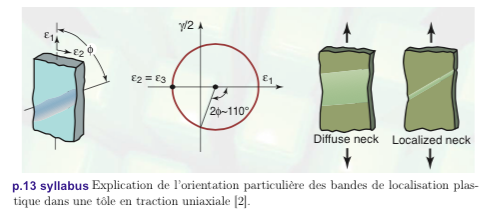
\includegraphics[scale=0.5]{mohr.png}
\caption{Cercle de Mohr}
\label{fig:mohr}
\end{figure}

\section{Chapitre II : Bases physique de la résistance mécanique des matériaux}
\subsection{Remarques}
\begin{itemize}[label=$\bullet$]
\item Un métal présentant de petits grains a une limite d'élasticité plus élevée car les joints sont des obstacles au déplacement des dislocations. $\to$ Il faut tirer plus pour entrer en plasticité.
\item Métal texturé : grains orientés préférentiellement dans une direction. La déformation plastique dans une direction favorise la réorganisation des grains et la formation d'un matériau texturé. (ex : laminage à froid)
\end{itemize}

\subsection{Définitions}
\begin{itemize}[label=$\bullet$]
\item Recristallisation : à haute température, une nouvelle génération de grains remplace au fur et à mesure les anciens par germination et croissance.
\begin{itemize}[label=$\hookrightarrow$]
\item Température de cristallisation : température à laquelle l'entièreté des grains sera recristallisée après une heure de traitement. Elle diminue si le matériau a un grande densité de dislocation. Au delà de cette température, le métal ne s'écrouit plus lorsqu'il est déformé plastiquement.
\end{itemize}
\item Restauration : réorganisation des dislocations en une configuration énergétique stable.
\item Martensite : pour le Fer, si la température est brutalement amenée d'une $T\degree ~> T\degree_{\textrm{allotropique}}$\footnote{Allotropie : faculté de certains corps simples d’exister sous plusieurs formes cristallines ou moléculaires différentes.} jusqu'à une $T\degree$ ambiante, la diffusion n'aura pas le temps de se faire et une phase dure et fragile (martensite) sera créée.
\end{itemize}

\section{Chapitre III : procédés de moulage des métaux}
\subsection{Donner 5 caractéristiques du moulage}
\paragraph{Avantages}
\begin{itemize}[label=$\bullet$]
\item Fabriquer en une seule opération des pièces à géométrie complexe.
\item Fabrication de pièces uniques (grandes) et pour production en série (usines, ...) $\to$ gain de temps.
\item S'applique à tous les métaux (favorisé si basse température de fusion) .

\end{itemize}

\paragraph{Désavantages}
\begin{itemize}[label=$\bullet$]
\item Propriétés mécaniques médiocres à causes des micro-structures.
\item Dimensions imprécises
\item Fini de surface grossier.
\end{itemize}

\subsection{Caractéristiques thermomécaniques}
\begin{itemize}[label=$\bullet$]
\item Point de fusion $T_m$
\item Quantité de chaleur libérée = chaleur latente de solidification $H_m$
\item Retrait de solidification $\Delta V_m$
\item Points chauds : zones refroidies trop lentement qui se retrouvent encapsulées à l'état fondu à l'intérieur du solide. $\to$ Cavités après solidification
\item Contraintes résiduelles (car équilibre)
\end{itemize}

\subsection{Germination vs croissance de grain}
\begin{itemize}[label=$\bullet$]
\item "Bon métal" si beaucoup de petits grains (joints = obstacles au déplacement des dislocations, ...)
\item Germination : $T\degree << T\degree_{fusion} \to$ trempe, bonne ductilité, ténacité en périphérie de la pièce. Refroidissement assez rapide que pour empêcher la croissance des grains
\item Croissance du grain : augmentation de la température
\end{itemize}


\subsection{Expliquer la solidification des métaux (alliages)}
\begin{itemize}[label=$\bullet$]
\item Les parois de l'empreinte du moule sont des sites préférentiels de solidification, d'une part, parce que les surfaces solides constituent des points d'ancrage des germes ; d'autres part parce que les parois sont plus froides que le métal fondu.
\item Métaux purs : germination sur les parois et croissance colonnaire ou "basaltique" des grains. Avec une frontière de solidification nette.
\item Alliages : la frontière de solidification est une zone pâteuse. Cela produit des dentrites, c'est à dire des cristaux squelettiques ramifiés comme les branches d'un arbre. Leur axe est dans une direction favorable à la croissance. (ex : Cu-Ni) (\textsc{figure} \ref{fig:Phase})


\begin{figure}[!ht]
\centering
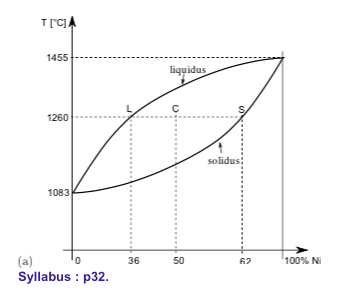
\includegraphics[scale=0.75]{Phase.png}
\caption{Diagramme de phase d'un alliage cuivre-nickel}
\label{fig:Phase}
\end{figure}


\item L'élément de l'alliage avec la plus haute température de fusion va se solidifier en premier $\to$ on aura dans le liquidus, du plus en plus de Cu ... composition hétérogène = \textbf{ségrégation}. Cela diminue la résistance du métal.
\item Ségrégation évitée avec alliages eutectiques (ex : Fe-C), ils passent directement de solide à liquide.
\end{itemize}

\subsection{Expliquer la viscosité}
L'aptitude du métal fondu à remplir l'empreinte du moule dépend de sa viscosité. Elle est mesurée en considérant 2 plaques planes séparées par un film fluide d'épaisseur homogène $h$. Le film fluide adhère aux parois et il oppose une résistance au déplacement d'une plaque par rapport à l'autre. La viscosité dynamique $\eta$ est le rapport de proportionnalité entre la contrainte nécessaire au mouvement et le gradient de vitesse à l'intérieur du film.
$$ \sigma_{12}= \dfrac{f}{A}= \eta \dfrac{dv_1}{dx_2}$$
où la contrainte de cisaillement $\sigma_{12}$ est obtenue en divisant la force $f$ par l'aire $A$ de la surface du film fluide. La viscosité dynamique se mesure donc en [Pa.s].

\subsection{Température initiale du bain fondu}
Une température élevée réduit la viscosité et facilite donc l'écoulement du fluide et le remplissage du moule. Cependant, la surchauffe implique aussi une plus grande quantité de chaleur à extraire, donc un refroidissement plus long que ce qui est strictement nécessaire et une microstructure plus grossière.

%Mise en page 
\pagebreak

\subsection{Comment remplir un moule ?}
Objectifs : remplissage complet de l'empreinte, éviter la ségrégation des éléments d'alliage, la porosité et la présence d'impuretés.
\begin{itemize}[label=$\bullet$]
\item Injection du métal sous pression pour vaincre la résistance au remplissage (gravité ou par centrifugation).
\item Débit limité afin d'assurer l'écoulement laminaire. Un écoulement turbulent augmente la surface de contact entre le fluide et l'air ambiant et donc l'incorporation au bain métallique d'agents contaminants.
\item Alimentation supplémentaire via les masselottes. ("veine" de métal continue, corrige la propagation du front de solidification et évite la formation de points chauds)
\item Ajout de refroidisseurs métalliques : sites préférentiels de germination et améliorent l'extraction de chaleur grâce à leur bonne conductivité thermique.
\end{itemize}

\subsection{Profils de température dans le moule, temps de solidification}
\begin{description}
\item[Equation à résoudre :] 
\begin{align*}
\rho c \dfrac{\delta T}{\delta t}&=k \dfrac{\delta^2T}{\delta x^2}\\
\end{align*}
Soit la diffusivité thermique :  $a = \dfrac{k}{\rho c}$ cette équation devient donc:
\begin{align*}
\dfrac{\delta T}{\delta t}&=a \dfrac{\delta^2T}{\delta x^2} 
\end{align*},  

\item[Solution :] $T(x,t) = T_m +(T_0 - T_m)erf \left( \dfrac{\xi}{2}\right)$ avec $\xi = x/\sqrt{at}$
\item[Hypothèses:] A la paroi de l'empreinte(x=0), la température $T_M$ est constante. \\
A la surface extérieure du moule,(x= -$\infty$), la température est aussi jugée constante et égale à $T_0$.	\\
La quantité de chaleur extraite est égale au flux de chaleur dégagé lors de la solidification.\\
nb: ok pour surfaces planes mais adaptées pour géométries diverses.
\item[Formule de Chvorinov :]
\begin{align*}
t_s &\cong \dfrac{\pi}{4}\left( \dfrac{\hat{\rho}H_m}{T_m -T_0}\right)^2 \dfrac{1}{\rho ck}\left( \dfrac{V}{A}\right)^2
\end{align*}
avec 
\begin{itemize}[label=$\bullet$]
\item $\hat{\rho}$ = la densité du métal
\item $\rho$ = la densité \textit{du moule ?}
\item $H_m$ = la chaleur latente de fusion.
\item A = surface totale
de l’empreinte du moule
\item V = le volume
\item c = la chaleur spécifique 
\item k = la conductivité thermique
\end{itemize}
\end{description}

%Mise en page
\pagebreak

\subsection{Conception d'un moule}
\begin{itemize}[label=$\bullet$]
\item Le moule doit avoir :
\begin{enumerate}
\item Une bonne tenue mécanique (même à haute T$\degree$)
\item Une bonne conductivité thermique + échappements pour chaleur, air et gaz (avec matériau poreux ou en usinant des évents au travers du moule)
\end{enumerate}
\item Deux types de moule : permanents (conicité minimale de la pièce) et à usage unique.
\item Pièce creuse : utilisation d'un noyau à l'intérieur de l'empreinte (soit en sable compacté qui se désagrège après moulage, soit en polystyrène qui s'évaporera au contact du métal chauffé), le noyau est maintenu par des supports intégrés à la pièce.
\item Surdimensionner le moule pour anticiper le retrait de solidification.
\end{itemize}
\textcolor{red}{Attention :} le noyau ne doit pas trop s'opposer au retrait, risque de fissure.

\subsection{Moules à usage unique}
Il existe deux procédés, le premier repose sur l'utilisation d'un \textbf{moule en sable compacté}. Il existe plusieurs sortes de sables : le sable vert, le sable grillé. Ils sont réalisés eux-mêmes par moulage à l'intérieur d'un châssis et autour d'un modèle dont la géométrie est celle de l'objet à mouler. Le moule est ouvrable pour extraire le modèle. On peut mélanger le sable à de la résine thermodurcissante, alors le moule peut lui-même prendre la forme d'une carapace ou d'un masque. Ce procédé est peu couteux, le sable peut résister à des hautes températures, si un sable fin est utilisé, le rendu de surface sera meilleur mais il diminuera la perméabilité du moule.
Le deuxième procédé,  \textbf{à modèle perdu}, consiste en un modèle réalisé en cire qui est extraite du moule à l'état fondu. Procédé couteux mais garantie d'une précision et d'un fini de surface.

\subsection{Moules permanents}
\begin{itemize}[label=$\bullet$]
\item Si utilisation du moules pour un grand nombre de pièces, il est réalisé dans un métal à haute température de fusion résistant à l'érosion (fonte, matériau réfractaire ou acier).
\item La surface de l'empreinte est recouverte d'un agent favorisant le détachement de la pièce moulée.
\item Procédé bien adapté aux métaux à faible point de fusion (comme alu).
\item Meilleure tenue mécanique : métal = bon conducteur, donc refroidissement rapide et microstructure plus fine.
\item Injection : aspiration sous-vide, gaz comprimé, gravité, centrifugation, pistons.
\item Noyau doit se désagréger.
\item Géométrie doit permettre le démoulage.
\item Pour les très grandes séries de pièces.
\item Pression additionnelle pour : augmenter la cadence de production ; améliorer le fini de surface.
\item Peut comprendre un système intégré de reffroidissement. 
\end{itemize}

%Mise en page
\pagebreak

\section{Chapitre IV : Procédés d'usinage}

Procédés utiles pour la \textbf{finalisation} de pièces de grande série ou pour la \textbf{fabrication} de petites séries de pièces.
\subsection{Avantages}
\begin{enumerate}
\item Tout type de forme peut être conféré à la pièce (procédé flexible).
\item Applicable à beaucoup de matériaux (sauf céramiques).
\item Outils peu coûteux (comparé au formage/moulage).
\item On peut atteindre des tolérances très élevées (centième de mm).
\item Convient très bien pour fabrication unique.
\end{enumerate}

\subsection{Inconvénients}
\begin{enumerate}
\item Gaspillage de matière (sauf si recyclage des copeaux).
\item Temps d'usinage plus long que le formage/moulage.
\item Fini de surface mauvais sauf si passes de finition (élévation du coût).
\end{enumerate}

\subsection{Paramètres de coupe}
\begin{enumerate}
\item Profondeur de passe (mm) : épaisseur retirée par passe.
\item Avance (par tour) (mm/t) tournage : déplacement de l'outil pour un tour de pièce.
\item Avance (mm/min) fraisage : vitesse de déplacement de l'outil.
\item Vitesse de coupe (m/min) : vitesse de l'outil lors de la coupe.
\item Vitesse de rotation (de broche) (t/min) : nombre de tours par minutes accomplis par la pièce lors de la coupe.
\end{enumerate}

\subsection{Formation de copeaux - Modèle de Merchant}

\paragraph{Hypothèses}
\begin{itemize}[label=$\bullet$]
\item Déformation plane
\item Copeau de section constante
\item Coupe en régime stationnaire
\item Le copeau est représenté comme plusieurs plans parralèlles glissant les uns sur les autres (paquet de cartes).
\end{itemize}

\paragraph{Relations d'angle}
\subparagraph{Paramètres}
\begin{itemize}[label=$\bullet$]
\item Angle de coupe orthogonal $\alpha$ (fixe cisaillement), angle de dépouille, angle de taillant, angle de cisaillement $\phi$
\item Épaisseur de coupe : $t_o$ (la profondeur de passe), $t_c$ (épaisseur du copeau) et rapport de coupe $r = \dfrac{t_o}{t_c} < 1$
\item Longueur du plan de cisaillement : $l_s$
\end{itemize}

\subparagraph{Développements :}
$$t_o = l_s \sin \phi$$
$$t_c = l_s \sin(90 -\phi+\alpha) = l_s \cos(\phi-\alpha)$$
$$\tan \phi = \dfrac{r\cos \alpha}{1-r\sin \alpha} $$

\begin{figure}[!h]
\centering
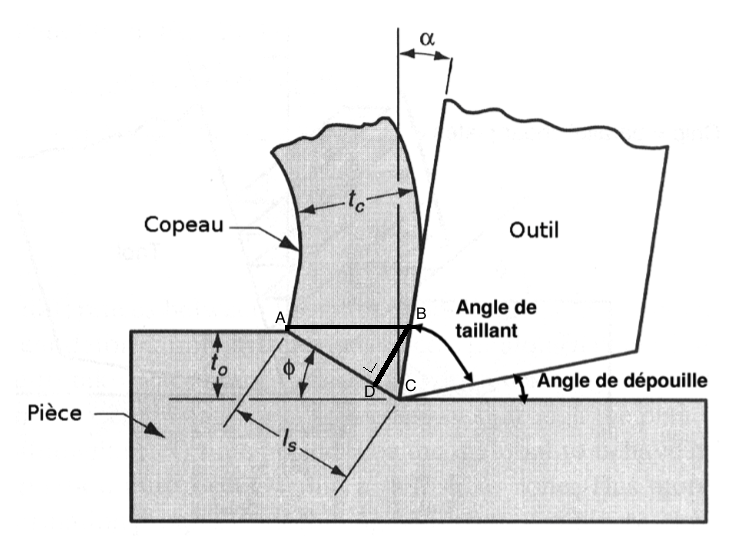
\includegraphics[scale=0.4]{Merchant.png}
\caption{Modèle de la coupe orthogonale de Merchant}
\label{fig:Merchant}
\end{figure}

\paragraph{Déformation par cisaillement}
$$\epsilon_{12} = \dfrac{AC}{BD}=\dfrac{AD+DC}{BD} = \tan(\phi-\alpha)+\cot\phi $$
Remarque : les frottements copeaux/outils induisent une deuxième zone de cisaillement, donc la température augmente et l'usure également.\\ 
Si $r$ augmente, et si $\alpha$ augmente, $\epsilon_{12}$ diminue.

\subsection{Force et puissance lors de la coupe}

\begin{figure}[!ht]
\centering
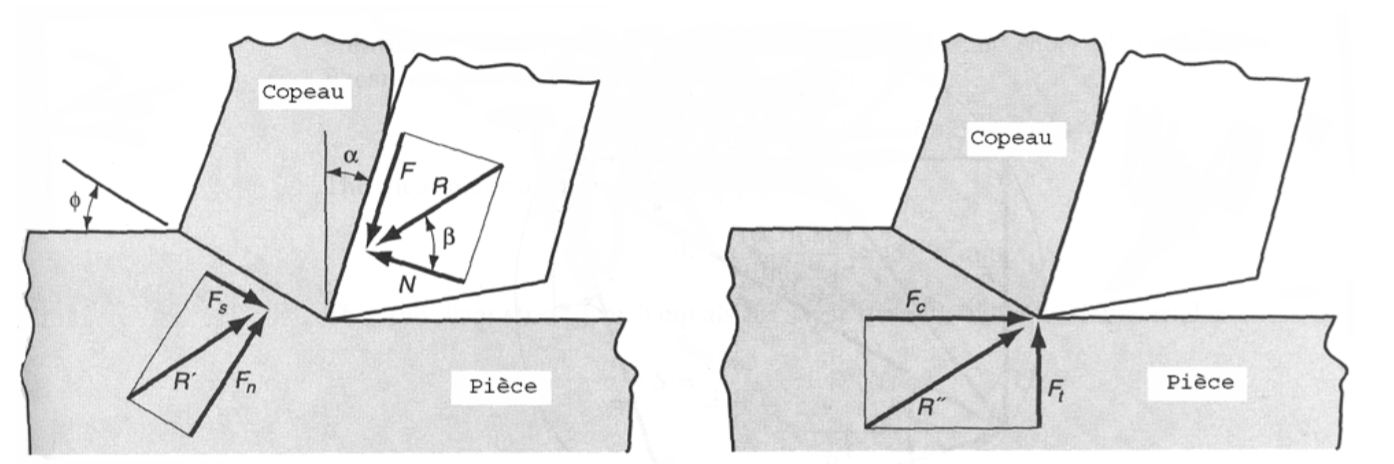
\includegraphics[scale=0.6]{MerchantFO.png}
\caption{Définition des Forces}
\label{fig:carreblanc3}
\end{figure}

\paragraph{Par l'outil :}
\begin{itemize}[label=$\bullet$]
\item Force de frottement F le long de la face de la coupe de l'outil et la force normale N.
\item Résultante de F et N, R, inclinée à un angle de frottement $\beta$

$\mu = \dfrac{F}{N}=\tan\beta$
\end{itemize}

\paragraph{Par la matière}
\begin{itemize}[label=$\bullet$]
\item $F_s$ Force de cisaillement, cause le cisaillement dans le plan de cisaillement.
\item $F_n$ Force normale au cisaillement qui lui est perpendiculaire.
\item $R'$ Résultante : $R' = -R$
\item Contrainte de cisaillement $\sigma_{12}$ :

$\sigma_{12} = \dfrac{F_s}{A_s}$ avec $A_s = \dfrac{t_0l_c}{\sin\phi}$ la surface du plan de cisaillement.
\item $F_c$ et $F_t$ sont les forces de coupe et d'avance
\end{itemize}
Les relations entre ces forces sont les suivantes :
\begin{align*}
  \left\{
  \begin{aligned}
      F & =F_c \sin \alpha + F_t \cos \alpha\\
      N & =F_c \cos \alpha-F_t \sin\alpha \\
      F_s & =F_c \cos\phi +F_t \sin\phi\\
      F_n & =F_c \sin\phi +F_t \cos\phi\\
      \sigma_{12} & =\dfrac{F_c \cos\phi-F_t \sin\phi}{A_s}
  \end{aligned}
  \right.
\end{align*}

\paragraph{Relation de Merchant}
Angle $\phi$ favorisé. Si $\alpha$ et $\eta$ augmentent, $t_c$ diminue et le copeau sera plus fin.
$$\dfrac{d\sigma_{12}}{d\phi} = 0 \rightarrow \phi = 45\degree +\dfrac{\alpha}{2}-\dfrac{\beta}{2}$$

\paragraph{Puissance de coupe :} $P_c= F_cV_c$, vu que le rendement $\eta$ est proche des 90\%, la puissance fournie par la machine est $P_f = \dfrac{P_c}{\eta}$

\paragraph{Énergie de coupe :} correspond au rapport entre la puissance de coupe et le volume coupé par unité de temps. 
\begin{align*}
E_c = \dfrac{F_c}{t_0l_c}=\dfrac{P_c}{V_ct_0l_c}
\end{align*}
 Par exemple, un acier au carbone requiert 2.8 J pour retire 1 mm$^3$ de matière alors qu'il ne faut que 0.8 J pour un alliage d'aluminium..
\subsection{Différents types de copeaux}
\paragraph{Copeau continu}
\begin{itemize}[label=$\bullet$]
\item Obtenu avec un matériau ductile, une haute vitesse de coupe ($V_c$), une faible avance, une faible profondeur de passe et/ou un large angle. Il y a donc peu de frottements entre l'outil et copeau. 
\item Bon état de surface.
\item Problème des longs copeaux : enroulement de celui-ci autour de l'outil (ce qui provoque un arrêt fréquent de la machine et compromet la sécurité de l'opérateur). Solution : brise-copeau sur l'outil.
\item Il peut y avoir une arête rapportée (adhésion de l'outil à la matière, processus cyclique). L'état de surface est altéré, après que l'arête se soit détachée.
\end{itemize}

\paragraph{Copeau discontinu}
\begin{itemize}[label=$\bullet$]
\item Obtenu avec un matériau fragile, et/ou avec une vitesse de coupe faible, et/ou avec un angle faible de coupe (Attention : inclusions dure, vibrations machines,..).
\item Copeau segmenté = irrégularité de la surface.
\end{itemize}

\subsection{Élévation de la température + causes et conséquences}
Lors du frottement outil/copeau, T = $700\degree$. La pièce reste relativement froide. 90$\%$ de l'énergie va dans le copeau (et dans l'outil). Si $V_c$ augmente, $T_{outil}$ augmente, $T_{copeau}$ augmente et $T_{pièce}$ diminue.
\paragraph{Causes}
\begin{itemize}[label=$\bullet$]
\item Travail fait par cisaillement dans la zone primaire de cisaillement.
\item Énergie dissipée en frottement dans la zone secondaire de cisaillement.
\item Énergie générée par le frottement de l'outil à la surface usinée si l'outil est usé. 
\end{itemize}

\paragraph{Conséquences}
\begin{itemize}[label=$\bullet$]
\item Limite d'élasticité, dureté et résistance de l'outil diminuent $\rightarrow$ longévité de l'outil altérée.
\item Dilatation thermique de l'outil $\rightarrow$ mauvaise précision dimensionnelle.
\item Changement de microstructure en surface de la pièce $\rightarrow$ modification des propriétés mécaniques.
\end{itemize}

\subsection{Où l'outil s'use-t-il ?}
\begin{itemize}[label=$\bullet$]
\item Facette parallèle à la vitesse de coupe
\item Cratère au contact outil/copeau
\end{itemize}
 Un outil usé ne respectera plus les tolérances dimensionnelles, il y aura plus de frottements et la température va donc augmenter.
\subsection{Quelles caractéristiques doit avoir l'outil ?}
\begin{enumerate}
\item Dureté élevée, même à chaud.
\item Résistant au fluage (déformation avec le temps).
\item Bonne ténacité, résistance à l'impact (pas de rupture à cause des vibrations.
\item Résistance à l'usure.
\item Résistance aux chocs thermiques.
\item Fait d'un matériau inerte (pas de réaction avec la pièce).
\end{enumerate}
$\longrightarrow$ Compromis entre dureté à chaud, ténacité, résistance à l'usure et prix.

\subsection{Quels sont les différents types d'outil ?}
\begin{enumerate}
\item Aciers rapides (durcis par trempe $\rightarrow$ martensite).
\item Carbure (frittage de poudres :  carbures et cobalt).
\item Outils revêtus ( cœur carbure + couche micrométrique en surface).
\item Céramique (vitesse de coupe haute, pas tenaces $\rightarrow$ pour la finition).
\end{enumerate}

\subsection{Que dire de l'état de surface ?}
Rugosité = différence de hauteur entre les points les plus hauts et les plus bas d'une surface.
\begin{itemize}[label=$\hookrightarrow$]
\item Élevée : faible tenue mécanique (surtout en fatigue).
\item Faible : temps d'usinage élevé (faible avance + passe de finition).
\end{itemize}

\subsection{Utilité du fluide de coupe ?}
\begin{enumerate}
\item Réduire la friction outil/pièce, diminution de l'usure.
\item Réduire la zone de coupe $\rightarrow$ résistance non-altérée.
\item Réduire la force de coupe (diminution de la friction), $\rightarrow$ diminution de l'énergie consommée.
\item Évacuation des copeaux si fluide sous pression.
\item Sectionner les copeaux.
\item Protège la surface de la machine de la corrosion.
\end{enumerate}

\subsection{Usinabilité}
L'usinabilité d'une matière est définie comme la capacité d'une matière à être travaillée par une machine-outil.
\paragraph{Dépend de :}
\begin{itemize}[label=$\bullet$]
\item Qualité de surface atteignable après usinage.
\item Durée de vie de l'outil.
\item Forces et puissances requises + utilisation fluide de coupe.
\end{itemize}

\paragraph{Exemples :}
\begin{itemize}[label=$\times$]
\item Aciers avec Al ou Si $\rightarrow$ oxydes $\rightarrow$ durée de vie diminue.
\item Ti : faible conductivité thermique.
\item Al : haut coefficient de dilatation thermique $\rightarrow$ dimensions !
\end{itemize}

\begin{itemize}[label=$\checkmark$]
\item Aciers avec élément à bas point de fusion $\rightarrow$ lubrification.
\end{itemize}

\subsection{Les différents procédés d'usinage}
\subsubsection{Tournage}
\paragraph{Caractéristiques :}
\begin{itemize}[label=$\bullet$]
    \item Mouvement de coupe circulaire donné à la pièce. L'outil se déplace.
    \item Axe des X radial ; axe des Z broche.
    \item Vitesse de coupe non constante car on fixe la vitesse de rotation.
\end{itemize}

\paragraph{Types :}
\begin{itemize}[label=$\bullet$]
    \item Tour parallèle : banc parallèle à Z où se trouve le chariot principal qui peut bouger dans le plan XZ.
    
    $\hookrightarrow$ Montage en l'air, soutenu par un mandrin (pour pièce courte) ; montage entre pointes (pour pièces longues) ; montage mixte (pour pièces plus lourdes).
    \item Tour vertical : pour pièces très lourdes.
\end{itemize}

\paragraph{Opérations :}
\begin{enumerate}
    \item Cylindrage/chariotage : cylindre extérieur.
    \item Tournage en cône.
    \item Dressage : fabriquer un plan normal $n_z$.
    \item Alésage : élargir un trou.
    \item Filetage : fabriquer un filet extérieur.
    \item Taraudage ou tour : fabriquer un filet intérieur.
    \item Saignage d'une gorge : si continuité, tronçonnage.
    \item Saignage d'une gorge à fond circulaire.
    \item Chanfreinage : casser une arête pour la rendre moins coupante.
\end{enumerate}

\begin{figure}[h!]
\centering
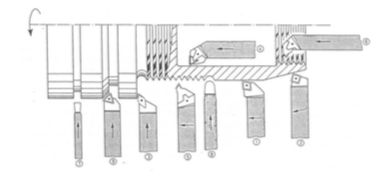
\includegraphics[scale=1]{tournage}
\caption{Opérations de tournage. p65 syllabus}
\end{figure}

\subsubsection{Rabotage}
\paragraph{Caractéristiques :}
Mouvement de coupe rectiligne.

\paragraph{Types :}
\begin{itemize}[label=$\bullet$]
    \item Raboteuse : mouvement de coupe donné à la pièce, mouvement d'avance et positionnement donnés à l'outil, réalisation de gorges rectilignes de grande précision.
    \item Étau-limeur : mouvement de coupe donné à une glissière (outil), mouvement d'avance discontinu donné à la pièce.
    \item Mortaiseuse : mouvement de coupe perpendiculaire à la table supportant la pièce, rainures et clavettes.
\end{itemize}

\begin{figure}[h!]
    \centering
    \begin{subfigure}[b]{0.3\textwidth}
        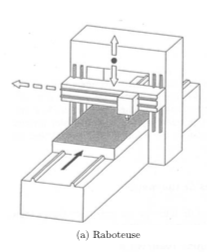
\includegraphics[width=\textwidth]{rabo.png}
        \caption{Raboteuse}
    \end{subfigure}
    ~ 
    \begin{subfigure}[b]{0.3\textwidth}
        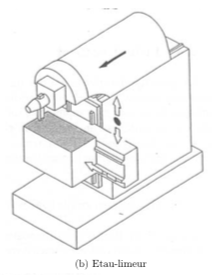
\includegraphics[width=\textwidth]{etau.png}
        \caption{Etau-limeur}
    \end{subfigure}
    ~ 
    \begin{subfigure}[b]{0.3\textwidth}
        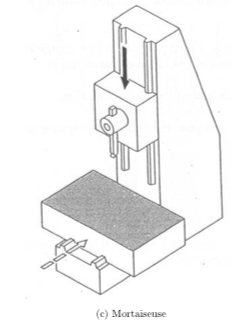
\includegraphics[width=\textwidth]{mort.png}
        \caption{Mortaiseuse}
    \end{subfigure}
    \caption{Machines à rabotage. p66 du syllabus}
    \label{fig:TOTAL}
\end{figure}


\subsubsection{Perçage - Forage}
\begin{itemize}[label=$\bullet$]
    \item Machine = perçeuse, outil = foret, mouvement de coupe circulaire.
    \item Permet taraudage et filetage mais passe de finition avec une aléseuse nécessaire.
    \item Brochage possible.
\end{itemize}

\subsubsection{Fraisage}
\paragraph{Types :}
\begin{itemize}[label=$\bullet$]
    \item Vertical : rotation de l'outil autour de Z, mouvement de la pièce dans XY (si mouvement possible "aléseuse-fraiseuse 3 axes).
    \item Horizontal : rotation de l'outil parallèle à XY, fraise en roulant mais ne facilite pas le changement d'outil.
\end{itemize}

\paragraph{Fonctionnement :}
\begin{itemize}[label=$\bullet$]
    \item En opposition : écarte la pièce de la table + vibration afin d'empêcher les copeaux de revenir sur la pièce.
    \item En avalant : plaque la pièce contre la table, précis et meilleur état de surface.
\end{itemize}

\subsubsection{Rectification}
Outil = meule faite de grains très durs qui vont abraser la surface de la pièce par enlèvement de micro-copeaux.

$\hookrightarrow$ Excellent état de surface, tolérance très serrée, usinage de matériaux durs.

\paragraph{Fonctionnement :}
Chaque grain retire une très faible quantité de matière. Les grains sont assemblés avec un liant en céramique ou ... Les pores entre les grains permettent le refroidissement et la formation de micro-copeaux.

\section{Chapitre V : Assemblages métalliques}
\subsection{Avantages du soudage}
\begin{itemize}[label=$\bullet$]
\item Jonctions étanches
\item Joint (parfois) plus résistant que les matières de base.
\item Peu coûteux.
\item Peut être réalisé sur le terrain pour les pièces de grande dimensions.
\end{itemize}

\subsection{Inconvénients}
\begin{itemize}[label=$\bullet$]
\item Main d'œuvre qualifiée coûteuse. (sauf pour grandes séries avec soudage automatisé).
\item Assemblage permanent.
\item Requiert beaucoup d'énergie.
\item Affaiblissement des propriétés mécaniques.
\item Contraintes résiduelles $\sim$ distorsion de la pièce ou rupture permanente.
\item Défauts de soudage difficiles à détecter 
\end{itemize}

\subsection{Définitions}
\begin{description}
\item[Intensité de puissance :] puissance transférée à la pièce par unité de surface [W/mm$^2$]. Temps nécessaire $\propto \dfrac{1}{I}$. Si l'intensité de puissance est faible, fusion impossible car chaleur perdue dans la pièce par conduction. Si l'intensité est trop élevée, risque d'évaporation du métal.
\item[Apport calorifique :] $H = P/v$, énergie transférée par unité de longueur du joint soudé [J/m]. Si l'apport est élevé, on parle de soudure chaude, et inversement. Pour que le joint soit sain, il faut souder avec $H$ le plus faible possible, pour cela on augmente la vitesse de coupe.
\item[Rapport de pénétration] = profondeur/largeur de la zone fondue.
\item[Dilution :] Proportion du matériau de base qui entre dans la constitution de la zone fondue composée du matériau de base et du matériau d’apport. Elle est nulle pour le \textbf{brasage} et non nulle pour le \textbf{soudage par fusion}.
\end{description}

%Mise en page
\pagebreak

\subsection{Les 4 zones de soudure}
\begin{figure}[!ht]
\centering
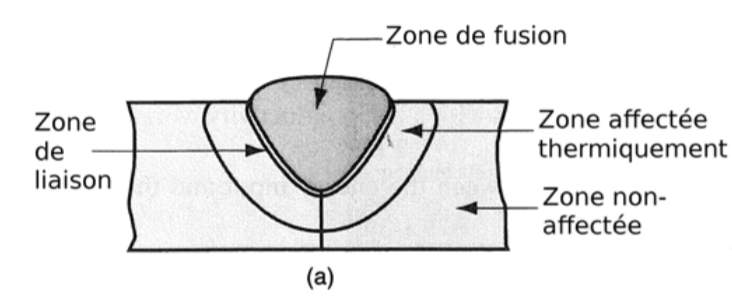
\includegraphics[scale=0.5]{Couches.png}
\caption{Les différentes zones du joint soudé}
\label{fig:couches}
\end{figure}

\paragraph{Zone Fondue}
Au centre du joint sous la source de chaleur. La composition chimique peut y être différente car apport de matière. Solidification à partir de grains existants, structure colonnaire (perpendiculaires à la direction des isothermes instantanés de fusion).

\paragraph{Zone de liaison}
Partiellement fondue, mais pas mélangée à la zone fondue, composition chimique du matériau de base.

\paragraph{Zone affectée thermiquement ZAT}
N'a pas atteint la température du solidus du matériau. La matière se restaure et se  recristallise $\rightarrow$ grains équiaxes très fins. MAIS près de la zone de fusion, la haute température a permis la recristallisassion, les grains sont donc plus grossiers.

\paragraph{Zone non-affectée}
Contraintes résiduelles suite à la contraction du bain fondu.

\textcolor{red}{Remarque : }si le matériau présente une transformation allotropique, les microstructures dans la ZAT sont donc plus complexes. Ex pour l'acier : si $T > T_{allo}$, une zone de transformation apparaît dans la ZAT. Dans cette zone, des grains fins apparaissent dû à la génération de la nouvelle structure cristallographique. Si refroidissement rapide, formation de martensite.

\subsection{Contraintes résiduelles}
\paragraph{Origine}
\begin{itemize}[label=$\bullet$]
\item Solidification $\rightarrow$ contraction transversale de la zone fondue (contraction de la pièce).
\item Après passage de la source de chaleur, la zone fondue se contracte longitudinalement et le reste de la pièce se dilate (traction au centre et le reste se dilate).
\end{itemize}

\paragraph{Éviter avant soudage :}
\begin{itemize}[label=$\bullet$]
\item Préchauffage : diminue les contraintes thermiques.
\item Puits thermiques pour évacuer rapidement la chaleur au niveau de la zone soudée.
\item Double passe (au dessus et en dessous).
\item Brider la pièce (restreindre le mouvement).
\end{itemize}

\paragraph{Éliminer après soudage :}
\begin{itemize}[label=$\bullet$]
\item Grenaillage : contrainte de compression au centre.
\item Mis sous tension de la structure soudée.
\item Traitement thermique.
\item On va également prendre en compte les caractéristiques de la pièce (fatigue, fluage, flambement, risque de rupture fragile, corrosion sous tension,...)
\end{itemize}

\subsection{Citer et expliquer les défauts du soudage}
\begin{enumerate}
\item\textbf{Porosités/soufflures} : dans la zones de fusion, petites bulles de gaz n'ayant pu s'échapper $\rightarrow$ souder des pièces propres et sèches, refroidissement plus lent ou postchauffe.
\item \textbf{Fissures} : zone de fusion ou dans le métal de base. Par exemple, si la matière d'apport n'a pas le même coefficient de dilatation thermique, risque d'apparition de fissures au refroidissement.
\item \textbf{Inclusions} : défaut si elles se rassemblent en bandes continues de matière non métallique (si utilisation de flux).
\item \textbf{Manque de fusion} : pas propagée à toute la section du grain.
\item \textbf{Manque de pénétration} : manque de fusion en profondeur ( =fissure, concentration de contraintes).
\item \textbf{Défauts de forme }: effondrement, retassure, concavité excessive ou débordement du cordon de soudure $\rightarrow$ concentration de contraintes.
\end{enumerate}


\begin{figure}[!htb]
\minipage{0.32\textwidth}
  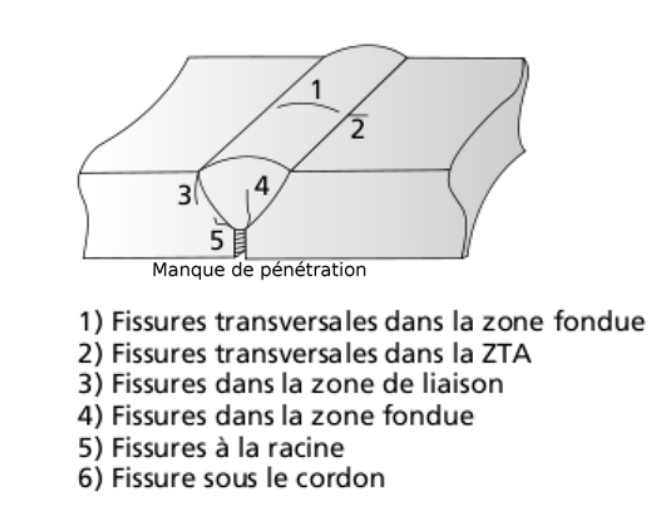
\includegraphics[width=\linewidth]{fissures.png}
  \caption{Fissures possibles}\label{fig:awesome_image1}
\endminipage\hfill
\minipage{0.32\textwidth}
  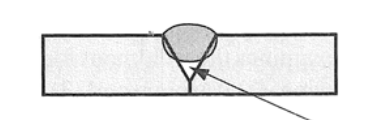
\includegraphics[width=\linewidth]{penetration.png}
  \caption{Manque de pénétration}\label{fig:awesome_image2}
\endminipage\hfill
\minipage{0.32\textwidth}%
  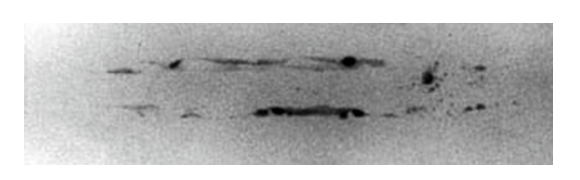
\includegraphics[width=\linewidth]{inclusion.png}
  \caption{Lignes d'inclusion dans la zone fondue}\label{fig:awesome_image3}
\endminipage
\end{figure}



\subsection{Comment détecter les défauts de soudure ?}
\paragraph{Techniques non-destructives}
\begin{itemize}[label=$\bullet$]
\item Ressuage : liquide teinté, persiste dans fissure après nettoyage.
\item Magnétique : poudre en surface, perturbée par les défauts.
\item Ultrasons : défauts $\rightarrow$ diminution de transmission du son.
\item Radiographie : rayon X ou gamma.
\end{itemize}

\paragraph{Techniques destructives}
\begin{itemize}[label=$\bullet$]
\item Analyse microscopiques d'échantillons.
\item Pliage à l'envers (manque de pénétration).
\end{itemize}

\subsection{Définir la soudabilité}
Capacité d'un métal ou d'une combinaison de métaux à être soudés dans la configuration souhaitée et tel que les joints résultants possèdent des propriétés mécaniques acceptables pour l'utilisation en service.

$\hookrightarrow$ Dépend de la technologie utilisée et des propriétés thermiques ($T_{fusion}$, conductivité thermique, coefficient d'expansion).

\subsection{Types de soudage par fusion}

\subsubsection{Soudure à l'arc}

\begin{itemize}[label=•]
\item Fusion assurée par un arc entre l'électrode et la pièce. L'arc électrique est entretenu par la formation d'un plasma(gaz ionisé).
\item Protection du bain indispensable, il en existe 2. La protection gazeuse (inerte ou active, crée une atmosphère oxydante) et la protection par flux (liquide recouvrant le bain fondu) qui doit être éliminé après le soudage.
\item Types de soudure à l'arc :
\begin{itemize}
\item Électrode consommable: source du matériau d'apport
\begin{enumerate}
\item Électrode enrobée $\rightarrow$ protection (gaz ou flux) fournie par l'enrobage de l'électrode.
% \begin{figure}[h!]
% \centering
% 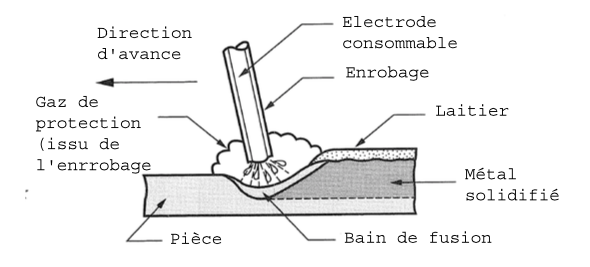
\includegraphics[scale=0.3]{enrob}
% \end{figure}
\item Fil fusible/semi-automatique. Métal d'apport en fil bobiné, gaz de protection.
% \begin{figure}[h!]
% \centering
% 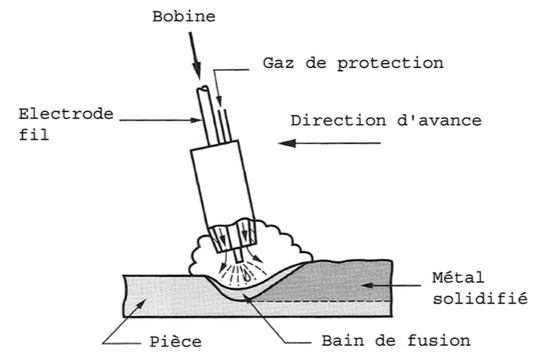
\includegraphics[scale=0.2]{fusible}
% \end{figure}
\item Avec fil fourré de flux : flux continu, à l'intérieur de l'électrode.
% \begin{figure}[h!]
% \centering
% 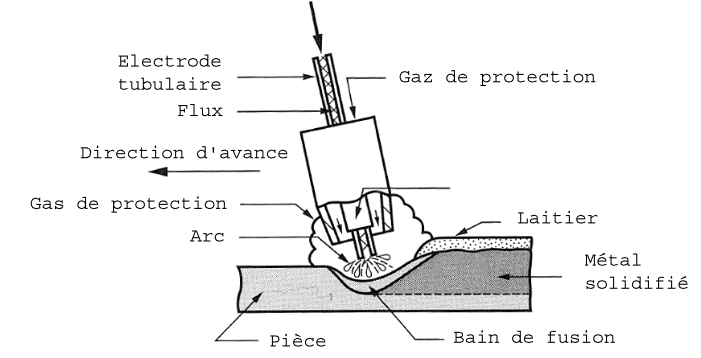
\includegraphics[scale=0.25]{flux}
% \end{figure}
\item Submergé : un fil se déroule pour alimenter automatiquement une zone fondue submergée dans le flux granulaire(favorise un refroidissement plus lent).
% \begin{figure}[h!]
% \centering
% 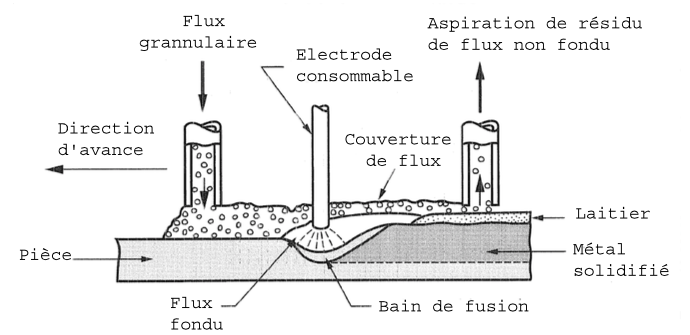
\includegraphics[scale=0.25]{submerge}
% \end{figure}
\end{enumerate}

\begin{figure}[h!]
    \centering
    \begin{subfigure}[b]{0.22\textwidth}
        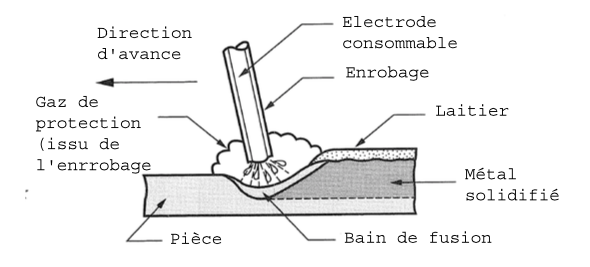
\includegraphics[width=\textwidth]{enrob.png}
        \caption{Soudage à l’arc avec électrode enrobée}
    \end{subfigure}
    ~ 
    \begin{subfigure}[b]{0.22\textwidth}
        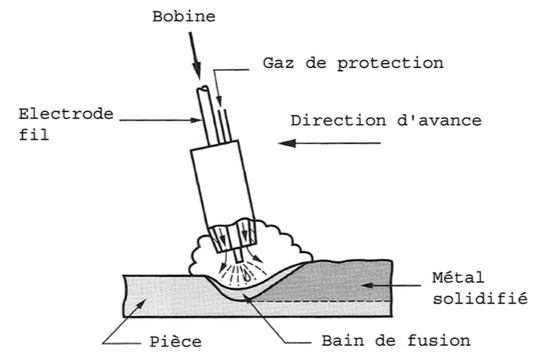
\includegraphics[width=\textwidth]{fusible.png}
        \caption{Soudage à l’arc avec fil fusible}
    \end{subfigure}
    ~ 
    \begin{subfigure}[b]{0.22\textwidth}
        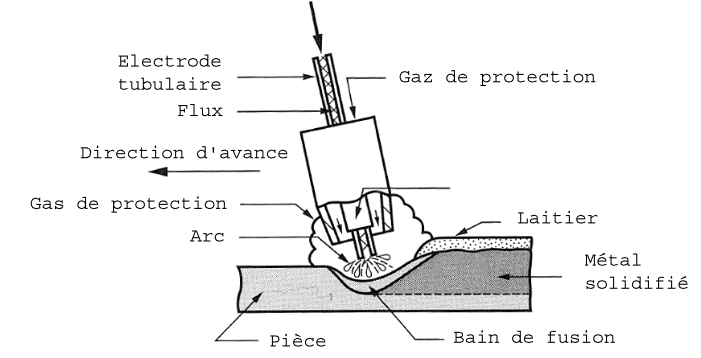
\includegraphics[width=\textwidth]{flux.png}
        \caption{Soudage à l’arc avec fil fourré de flux}
    \end{subfigure}
    ~
    \begin{subfigure}[b]{0.22\textwidth}
        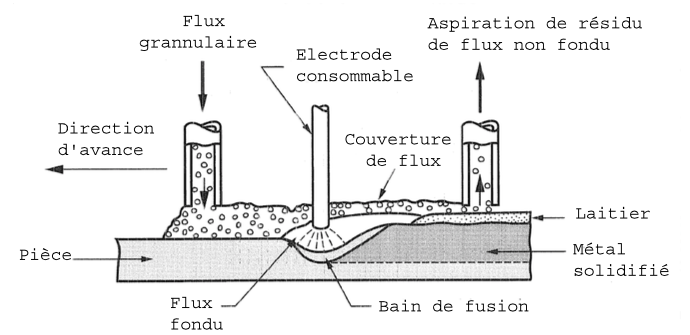
\includegraphics[width=\textwidth]{submerge.png}
        \caption{Soudage à l’arc submergé}
    \end{subfigure}
\end{figure}

\item Électrode non-consommable: souvent en Tungstène ($T_{fusion}$très élevée), un matériau d'apport doit être fourni séparément.
\begin{enumerate}
\item Électrode réfractaire du tungstène (TIG): protection gazeuse fournie indépendamment. Sans métal d'apport ou baguette indépendante avec métal d'apport.
\begin{figure}[h!]
\centering
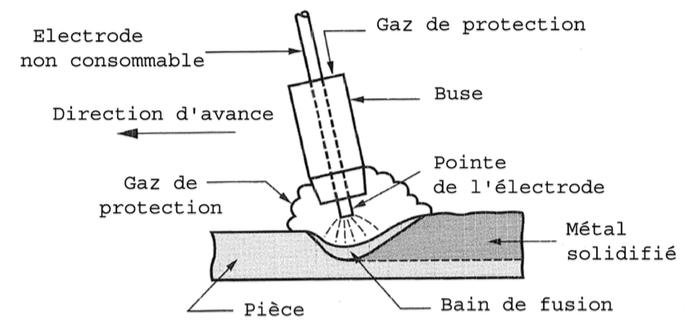
\includegraphics[scale=0.3]{tig.png}
\caption{Soudage TIG}
\end{figure}
\item Au plasma : électrode de tungstène à retrait pour ioniser le gaz de protection. la température augmente très fortement : intensité de puissance très élevée, on peut augmenter la vitesse d'avance.
\begin{figure}[h!]
\centering
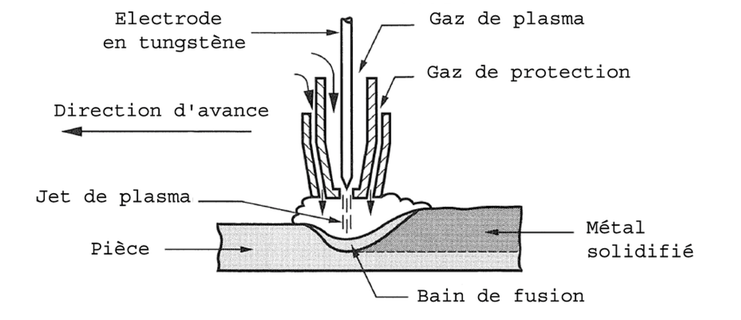
\includegraphics[scale=0.3]{plasma.png}
\caption{Soudage au plasma}
\end{figure}
\end{enumerate}
\end{itemize}
\end{itemize}
% \begin{figure}[h!]
%   \centering
%   \subfloat[Soudage TIG]{\label{fig:A}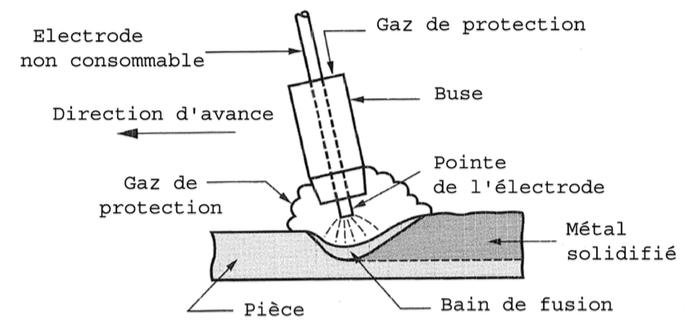
\includegraphics[scale=0.3]{tig}}
%   \hspace{.1pt}
%   \subfloat[Soudage au plasma]{\label{fig:B}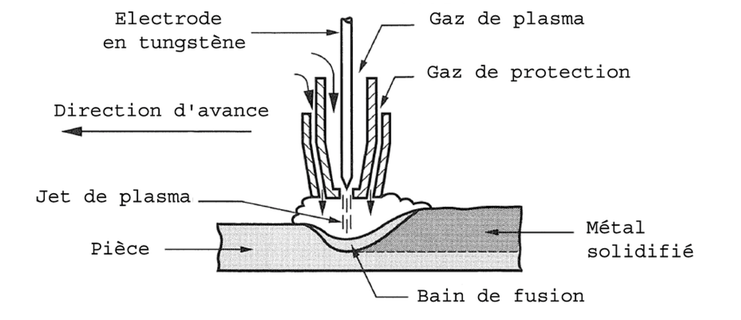
\includegraphics[scale=0.3]{plasma}}
% \end{figure}


\subsubsection{Soudure au gaz : source de chaleur = réaction chimique}
\begin{itemize}[label=$\bullet$]
\item Réaction primaire : $2C_2H_2 + 2O_2 \rightarrow 4CO + 2H_2 + \text{ chaleur}$
\item Réaction secondaire : $4CO + 2O_2 \rightarrow 4CO_2 $, protection gazeuse du bain fondu.
\begin{figure}[h!]
\centering
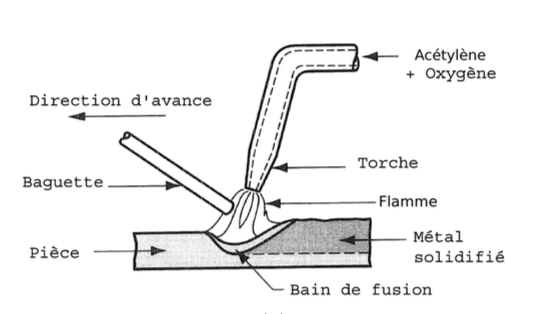
\includegraphics[scale=0.3]{gaz.png}
\caption{Soudage au gaz}
\end{figure}
\end{itemize}

%Mise en page
\pagebreak

\subsubsection{Soudage par résistance}


$\hookrightarrow$ Application d'un courant à travers un assemblage de 2 plaques empilées. Avantages: pas de flux/gaz de protection, peut être automatisé. Inconvénient : usure rapide $\rightarrow$ surcoût.

\begin{figure}[!ht]
\centering
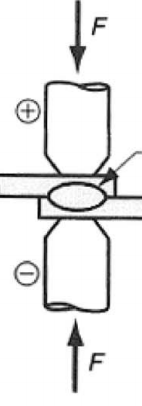
\includegraphics[scale=0.35]{soudageRes.png}
\caption{Soudage par résistance}
\label{fig:res}
\end{figure}


\subsubsection{Soudure au laser/faisceau d'électrons}
L'intensité est très élevée, donc on aura un bon rapport de pénétration pour des grandes vitesses d'avance. On aura la formation d'une capillaire pour une meilleure profondeur de pénétration.


\subsection{Soudage en phase solide}

\subsubsection{Technologies}
\begin{enumerate}
\item Diffusion : 2 surfaces de faible rugosité pressées et chauffées. Rétablissement de la liaison mécanique
\item Friction : échauffement par rotation puis pression $\rightarrow$ joint.
\item Ultrasons : 2 pièces frottant l'une contre l'autre à la fréquence des ultrasons, peu d'échauffement. Couche d'oxyde cassée $\rightarrow$peu d'échauffement, on peut souder des matériaux avec des grandes températures de fusion.
\item Co-laminage : pression et déformations cassent la couche d'oxyde en surface des deux tôles $\rightarrow$ assure le contact métal-métal.
\item Par explosion : Jet de plasma éjecté $\rightarrow$ surface nettoyée !
\end{enumerate}

\begin{figure}[!ht]
\centering
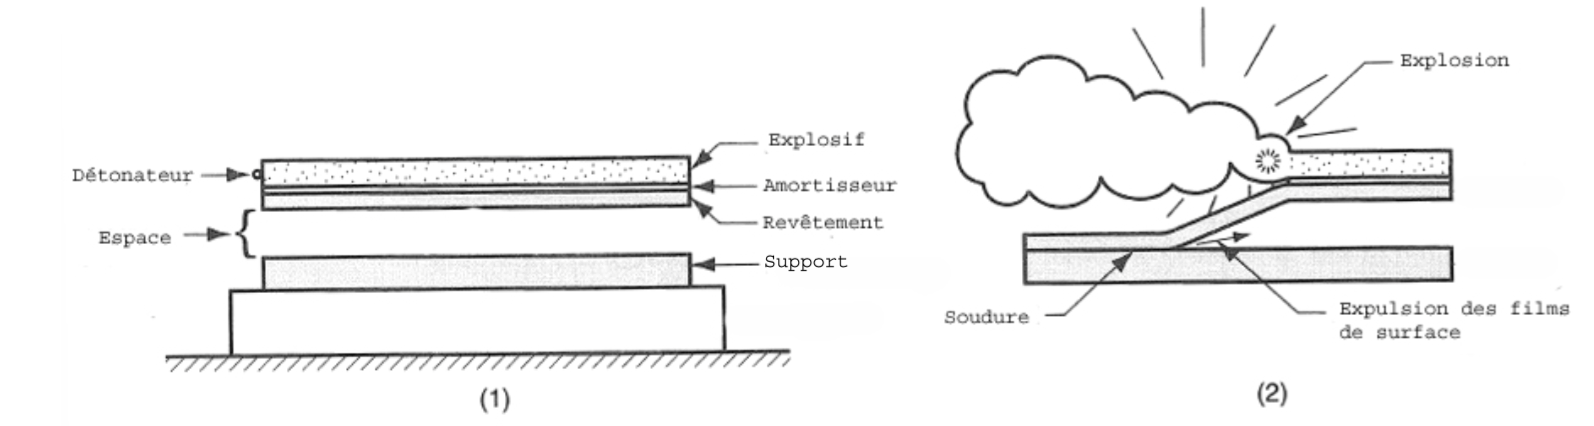
\includegraphics[scale=0.5]{Explosion.png}
\caption{Soudage par explosion}
\label{fig:explosion}
\end{figure}

\subsubsection{Avantages du soudage à l'état solide :}
\begin{enumerate}
\item Soudage dissimilaire $\rightarrow$ deux métaux, alliages différents,..
\item Bonnes propriétés mécaniques
\item La géométrie s'y prête bien
\end{enumerate}

\subsection{Expliquer le brasage}
\paragraph{Concept :}
Surfaces nettoyées par un solvant $\rightarrow$ bonne mouillabilité. Il est assuré par un métal d'apport qui est placé entre deux surfaces à assembler et, après élévation de la température, fond et pénètre à l'interface entre les pièces à assembler par capillarité. Brasage fort : $T_{fus mat}\ge 450\degree$C. Brasage faible : $T_{fus mat}\le 450\degree$C.
\paragraph{Technologie :} Torche à gaz et chauffage par induction ou résistance
\paragraph{Avantage :}
ZAT beaucoup moins grande que par fusion.

\paragraph{Favorisé (il vaut mieux braser que souder quand):}
\begin{itemize}[label=$\bullet$]
\item Faible soudabilité du métal.
\item Assemblage de métaux dissimilaires qui sont difficilement soudable par fusion.
\item La géométrie de la pièce n'est pas propice au soudage, géométries complexes.
\item Une résistance élevée de l'assemblage n'est pas requise.
\end{itemize}

\subsection{Propriétés d'un bon matériau d'apport pour le brasage}
\begin{itemize}[label=$\bullet$]
\item Faible température de fusion.
\item Faible tension de surface.
\item Bonne fluidité pour pénétration par capillarité.
\item Aucune interaction chimique ou physique avec le métal de base.
\end{itemize}

\subsection{Avantages du collage}
\begin{itemize}[label=$\bullet$]
\item Applicable à une large gamme de matériaux (et aux assemblages dissimilaires).
\item Joint flexible après curage.
\item Curage demande peu d'énergie($T_{curage}<<<T_{fusion}$), ne change pas la microstructure.
\item Joint étanche.
\end{itemize}

\subsection{Inconvénients du collage}
\begin{itemize}[label=$\bullet$]
\item Température de service limitée.
\item Reproductibilité difficile à assurer.
\item Curage : temps parfois long, baisse productivité.
\item Joint collé souvent moins résistant que soudure.
\item Liaisons inter-atomiques différentes de celle du matériau de base.
\item Nécessité de préparer les surfaces à coller.
\end{itemize}

\subsection{Critère de bonne qualité ? Tenue mécanique des joints pour différents modes de chargements ?}
Bonne qualité : rupture dans la colle et non à l'interface.

Mode de chargement : meilleure tenue au cisaillement ou à la tension qu'au clivage ou au pelage.

\subsection{Deux types de colle}
Naturelle (collagène) : résistance du joint collé n'est pas requise ou grande surface de colle.

Synthétique : polymères thermoplastiques ou thermodurcissables, utilisation industrielle.

\pagebreak

\section{Chapitre VI : Mise en forme par corroyage}
\subsection{Introduction}
Procédés visant une déformation plastique (donc irréversible) du matériau. Pour rappel, une déformation est dite plastique si les sollicitations sont supérieures à un niveau de contrainte nommé "limite d'élasticité". On dit qu'une déformation est \textit{visco-plastique} si la réponse du matériau dépend en plus de la vitesse. Ce procédé confère une bonne tenue mécanique à la pièce mise en forme.
\subsection{Déformation (visco) plastique à l'état solide}
\begin{itemize}[label=$\bullet$]
\item Amplitude de déformation limitée
	\begin{itemize}[label=$\rightarrow$]
		\item Métaux malléables : peu résistants et ductiles
        \item Pré-chauffage tiède ou à chaud (mais oxydation, rugosité, usure des outils)
	\end{itemize}
    \item Pièces produites très résistances et anisotropes
\end{itemize}
\subsection{A quels métaux s'applique cette technique ?}
$\rightarrow$ A la majorité des métaux et alliages. 

Idéalement il faut :
\begin{itemize}[label=$\bullet$]
\item Limite d'élasticité faible.
\item Ductilité importante.
\item Préchauffer les matériaux peu malléables.
\item Traitement thermique de restauration après corroyage.
\end{itemize}

\subsection{Expliquer le forgeage}
C'est l'écrasement d'un lopin (volume) de matière en plusieurs étapes. Cela donne lieu un à écrouissage progressif de l'ébauche.
\begin{itemize}[label=$\bullet$]
\item Le lopin est soumis à des efforts de compression (via marteau ou presse).
\item Souvent préchauffé à haute température.
\item Forgeabilité maximum quand le lopin se déforme juste au dessus de sa température de recristallisation.
\item Les dernières frappes (à + faible température) affinent la microstructure (réduisent la taille des grains) + améliorent la précision dimensionnelle.
\end{itemize}

%Mise en page
\pagebreak

\subsection{A quoi reconnaît on une pièce forgée ?}
\paragraph{Point de vue microscopique :}
Grains et inclusions sont alignés avec la direction d'extensions maximale. Résistance et ténacité excellentes dans la direction des fibres, médiocres transversalement. Taux de corroyage = $\dfrac{A_{finale}}{A_0}$ limité pour éviter la fissuration le long des joints de grains(entre 3 et 8).

\paragraph{Point de vue macroscopique :}
Géométrie 3D, bonne tenue mécanique.

\subsection{Expliquer la frappe avec marteau}
Succession d'impacts avec un marteau (ou mouton) accéléré en chute libre ou par propulsion d'air (marteau pilon). L'énergie cinétique est convertie en énergie de déformation dans le lopin, le marteau et les fondations : 
\begin{align*}
\dfrac{1}{2}m_{\text{marteau}}v_{\text{marteau}}^2 &= \displaystyle{\int_{\Omega_L}^{}}\int_{0}^{\varepsilon^{tot}_{eq}}~ \sigma_{eq}d\varepsilon_{eq}d\Omega + \displaystyle{\int_{\Omega_F}^{}}\int_{0}^{\varepsilon^{tot}_{eq}}~\sigma_{eq}d\varepsilon_{eq}d\Omega
\end{align*}
\begin{itemize}[label=$\bullet$]
\item Le lopin est déformé car énergie emmagasinée sous forme élastique plus faible.
\item L'énergie nécessaire augmente avec la rigidité.
\item Lopin ductile car matière sollicitée en compression et de part la température élevée.
\item Si réponse viscoplastique (métal) à haute température $ \rightarrow$ utiliser une presse.
\end{itemize}

\subsection{Expliquer le forgeage avec une presse}
\begin{itemize}[label=$\bullet$]
\item Permet une déformation plastique jusqu'au coeur (lent).
\item Force $\propto$ à la section max et aux frottements.
\item Types : presse mécanique : axe en rotation fait descendre l'outil en mouvement rectiligne $\rightarrow$ taux de productivité élevé, régime constant. Presse hydraulique : huile sous pression ($F_{max} \propto F_{pompe}$) $\rightarrow$ coûteux.
\item Surfaces libres bombées car frottement + outil froid $\rightarrow$ diminution de la déformation au contact de l'outil. Deux solutions : la lubrification (diminution des frottements, augmentation de l'isolation thermique) et préchauffer les outils (forgeage isotherme).
\end{itemize}

\subsection{Solution approchée de la force de compression + hypothèses}
\paragraph{Hypothèses}
\begin{enumerate}
\item Lopin cylindrique en compression axi-symétrique.
\item Comportement isotrope du métal.
\item L'amplitude des déformations élastiques est négligeables par rapport aux déformations plastiques.
\item Frottement $\rightarrow$ cisaillement au contact des outils.
\item Cisaillement négligeable hors de la zone de frottement.
\item Limite d'élasticité homogène à travers le lopin.
\end{enumerate}

\paragraph{Solution}
\begin{align*}
F &: \sigma_{y}^2\left(1+m\dfrac{2R}{3h}\right)
\end{align*}

\subsection{Forgeage libre}
\begin{itemize}[label=$\bullet$]
\item L'ébauche a beaucoup de surfaces libres.
\item Refoulement : réduction de la hauteur du lopin.
\item Rétreinte : réduction locale de la section du lopin.
\item Martelage rotatif : ébauches de sections circulaires.
\item Poinçonnage : formation d'un trou.
\item Diminuer la longueur : à l'aide d'un couperet.
\end{itemize}

\subsection{Forgeage en matrice fermée}
Estampage = 2 matrices gravées se ferment et forcent le métal à remplir l'empreinte.
\begin{enumerate}[label=\alph*)]
\item Courber la pièce selon la courbure du produit fini.
\item Répartir la masse selon l'axe de l'ébauche.
\item Mettre en forme au fur et à mesure (de moins en moins d'arrondis aux angles).
\item Ébavurer la pièce.
\end{enumerate}
Ces étapes améliorent le fibrage et diminuent l'usure des outils.

\subsection{Extrusion vs tréfilage}
\begin{itemize}[label=$\bullet$]
\item Extrusion : produit des pièces allongées de section constante, appelées profilés.
\item Tréfilage : longs fils ou câbles de section circulaire.
\end{itemize}
Leur point commun est la mise en forme par écrasement lors du passage dans une filière.

\paragraph{Extrusion}
\begin{itemize}[label=$\bullet$]
\item Compression en direct, piston.
\item A chaud, à tiède ou à température ambiante.
\end{itemize}

\paragraph{Tréfilage}
\begin{itemize}[label=$\bullet$]
\item Traction en aval (+ étirage).
\item Température ambiante $\rightarrow$ meilleure résistance, meilleure précision dimensionnelle.
\end{itemize}

%Mise en page
\pagebreak

\subsection{Angle optimal de filière}
\paragraph{Enjeu :}minimisation de l'énergie de mise en forme.
\paragraph{Hypothèses :}
\begin{enumerate}
\item Filière section circulaire.
\item Rayon initial et final connus.
\item Angle d'entrée inconnu. 
\item Conservation matière, $V_{out}=V_{in}$
\end{enumerate}

\paragraph{Trois contributions à la puissance dissipée :}
\begin{enumerate}
\item $\dot{W}_{min}=$ déformation du lopin selon le trajet le plus direct.

$\dot{W}_{min}= \dot{Q}\overline{\sigma}_y2\ln \left( \dfrac{R_{in}}{R_{out}} \right) $
\item $\dot{W}_{red}=$ déformation plastique redondante. 

$\dot{W}_{red}= \dfrac{2\overline{\sigma}_y}{\sqrt{3}}\dot{Q}\dfrac{\alpha-\cos\alpha\sin\alpha}{\sin^2\alpha}$
\item $\dot{W}_{fr}=$ frottement contre la filière. 

$\dot{W}_{fr}=\dfrac{2\tau \dot{Q}}{\sin\alpha\cos\alpha}\ln\left( \dfrac{R_{in}}{R_{out}} \right)$
\end{enumerate}

\paragraph{Résultante}
\begin{align*}
\dfrac{F}{A} = \sigma_{zz} &= \dfrac{\dot{W}_{min}+\dot{W}_{red}+\dot{W}_{fr}}{\dot{Q}}\\
 &= 2\overline{\sigma}_y\left(\dfrac{\alpha-\cos\alpha\sin\alpha}{\sqrt{3}\sin^2\alpha}+\left(A+\dfrac{m}{\sin\alpha\cos\alpha}\right)\ln\left(\dfrac{R_{in}}{R_{out}}\right) \right)
\end{align*}

Optimisé pour $\alpha \approx 15\degree$.

\subsection{Contraintes techniques de la production}
\begin{itemize}[label=$\bullet$]
\item Section finale $<<<$ section initiale  $\rightarrow$ plusieurs passes + positionnement de recuits\footnote{rappel: permet la réchauffe du métal et maintient au-dessus de sa température de recristallisation pour activer des processus de diffusion qui restaurent la ductilité.} si capacité d'écrouissage épuisée.
\item Taux de réduction : $\rho = (A_{in}-A_{out})/A_{in}$. $F\propto \rho$ : il faut limiter les efforts. (F augmente $\rightarrow$ usure, température augmente)
\item Lent si métal résistant : il faut laisser diffuser la chaleur.
\item Échauffement $\rightarrow$ hétérogénéités en surface, ne doivent pas être trop grandes sinon gauchissement pour des profilés non-symétriques.
\item Tréfilage et étirement : risque de striction\footnote{Concentration des déformations plastiques en un endroit jusque rupture} quand le métal a épuisé sa capacité d'écrouissage.
\end{itemize}

\subsection{Laminage de produits plats}
Passage (écrasement) d'un lopin de métal entre deux rouleaux tournant en sens opposés. Permet de faire des poutres tubes, feuilles d'acier destinées à l'emboutissage, ... Technologie incrémentale : d'abord à température élevée puis à température ambiante, cela provoque une meilleure résistance, un contrôle dimensionnel, et un fini de surface. Pratique pour production de masse.

\subsection{Écoulement plastique induit par laminage}
\textsc{Voir feuille manuscrite. Camille ?}

Pour une compression plane :

\begin{align*}
\dot{\varepsilon}_{xx}^{pl} = -\dot{\varepsilon}_{zz}^{pl} \quad &\text{et} \quad \dot{\varepsilon}_{yy}^{pl} =0\\
\tilde{\sigma}_{xx} =- \tilde{\sigma}_{zz} \quad &\text{et} \quad \tilde{\sigma}_{yy} = 0
\end{align*}

En prenant compte du critère de Von Mises, on obtient :
\begin{align*}
\sqrt{\dfrac{3}{2}(\tilde{\sigma}_{xx}^2+\tilde{\sigma}_{zz}^2)} &= - \sqrt{3} \tilde{\sigma}_{zz} = \sigma_y\\
\Rightarrow \sigma_{zz}-\sigma_{xx} &= \tilde{\sigma}_{zz} - \tilde{\sigma}_{xx} = 2 \tilde{\sigma}_{zz} = - \dfrac{2}{\sqrt{3}}\sigma_y
\end{align*}

Si on fait hypothèse que la contrainte axiale est très petite par rapport à la contrainte d'écrasement ($|\sigma_{xx}|<<<|\sigma_{zz}|$), on en déduit que la puissance dissipée lors de la compression plane est supérieure à celle qui serait dissipée lors d'une compression uni-axiale.
\begin{align*}
\dot{W}_{\text{def}} = \sigma_{ij}\dot{\varepsilon}_{ij}^{pl} &= - \dfrac{2}{\sqrt{3}}\bar{\sigma}_y \dot{\varepsilon}_{zz}^{pl} \quad \text{si} \quad \dot{\varepsilon}_{yy}^{pl}= 0\\
&= -\bar{\sigma}_y \dot{\varepsilon}_{zz}^{pl} \quad \text{si} \quad \sigma_{yy} = 0
\end{align*}

Les raisons pour lesquelles on lamine quand même par une déformations planes sont les suivantes :

\begin{enumerate}
\item Analogiquement au forgeage, le frottement tend à empêcher un élargissement du lopin selon la direction de l'axe des rouleaux (\textbf{e}$_y$)
\item La seconde raison est qu'un allongement selon \textbf{e}$_y$ ne peut se faire sans entraîner la partie du lopin en amont des rouleaux ce qui n'est pas le cas selon \textbf{e}$_x$
\end{enumerate}

\begin{wrapfigure}{r}{60mm} 
  \centering
  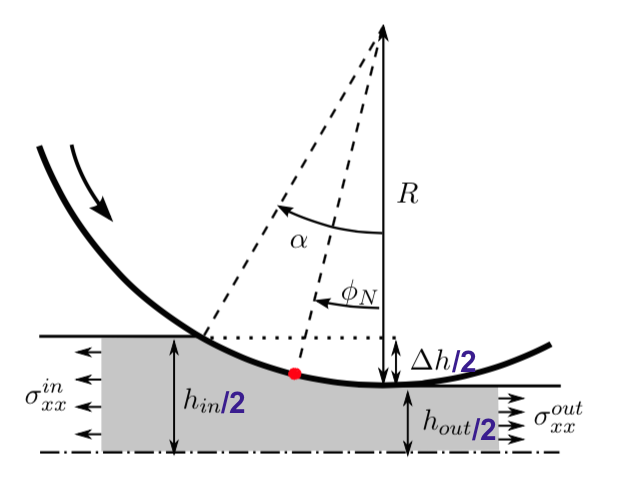
\includegraphics[scale=0.3]{laminage.png}
  \caption{Géométrie du laminage}
\end{wrapfigure}

\paragraph{Frottements}
 Les frottements ont une grande importance dans le laminage, en effet sans ceux-ci les rouleaux glisseraient sur la surface du lopin qui resterait immobile et il n'y aurait pas de laminage.
 
\subparagraph{Limite de la réduction}
Selon le schéma ci-contre, le lopin est poussé vers la droite si 
\begin{align*}
\int^\alpha_0 \mu p(\phi) \cos(\phi) w d\phi &\geq \int^\alpha_0 p(\phi) \sin(\phi) w d\phi
\end{align*}
Cette inégalité est vérifiée pour tout profil de pression $p(\phi)$ exercé sur l'interface à condition que 
\begin{align*}
\forall \phi \leq \alpha &, \quad \mu \geq \dfrac{\sin(\phi)}{\cos(\phi)}
\end{align*}

C'est à dire si $\mu \geq \tan(\alpha)$, et vu que 
\begin{align*}
\cos(\alpha) &= \dfrac{R-\frac{\Delta h}{2}}{R} = 1 - \dfrac{\Delta h}{2R}
\end{align*}

Dès lors, 
\begin{align*}
\tan(\alpha) = \dfrac{\sqrt{1-\cos{(\alpha)}^2}}{\cos(\alpha)} = \sqrt{\dfrac{\Delta h}{R}} \dfrac{\sqrt{1-\dfrac{\Delta h}{4R}}}{1-\dfrac{\Delta h}{2R}} \cong \sqrt{\dfrac{\Delta h}{R}} \qquad \text{si} \quad \dfrac{\Delta h}{2} << R
\end{align*}
Ce qui donne :
\begin{align*}
\rho &= \dfrac{\Delta h}{h_{in}} = \dfrac{h_{out}-h_{in}}{h_{in}} \leq \dfrac{R}{h_{in}} \mu^2
\end{align*}
Soit la conservation du volume et donc du flux de matière :
\begin{align*}
\dot{Q} = v_{in} w h_{in} = v_{out} w h_{out} \quad &\text{et} \quad \dfrac{v_{out}}{v_{in}} = \dfrac{h_{in}}{h_{out}}
\end{align*}
On peut donc en conclure que le métal \textbf{accélère lorsqu'il passe sous les rouleaux}.

Puisque le frottement s’exerce dans la direction de la vitesse relative de la surface du rouleau par rapport au lopin, le lopin n’est entraîné par les rouleaux que si :

\begin{align*}
v_{in} \cos(\alpha) \leq \omega R
\end{align*}
\subsection{Pilotage d'un laminoir}
Lorsque plusieurs laminoirs travaillent en tandem, il faut synchroniser les vitesses pour éviter l'opposition de contraintes. Des tendeurs mesurent $\sigma_{xx}^{in}$ et $\sigma_{xx}^{out} \rightarrow$ ils influencent la position du point neutre et l'amplitude de $F$.

Point neutre : le métal accélère lors de son passage dans le laminoir et sa vitesse peut être supérieure à la vitesse circonférentielle. Il existe un point (dit neutre) où la vitesse d'entrée est égale à $\omega R$.

\subsection{Problème rencontrés lors du laminage}
\begin{enumerate}
\item Déflexion élastique de l'axe des rouleaux due aux efforts de flexion. Solution : réduire rayon des rouleaux, leur donner une forme bombée.
\item Écrasement au centre plus ou moins fort que celui sur les bords. Cela donne lieu à des contraintes résiduelles importantes qui peuvent être relâchées par flambement ou par fissuration.
\item Les bords latéraux sont libres, il y a donc un risque d'allongement selon $e_z$, qui peut être compensé en partie par un élargissement de la tôle selon l'axe $e_y$.
\end{enumerate}

\subsection{Expliquer le pliage}

\begin{itemize}
\item Problème principal = RETOUR ÉLASTIQUE $\rightarrow$ plier d'avantage.
\item Hypothèses : couple pur, absence d'effort tractant. (selon l'épaisseur, contrainte de cisaillement moyenne nulle)
\item Après pliage, les fibres matérielles forment des arcs concentriques. Rayon intérieur, fibres raccourcies ; rayon extérieur, fibres allongées ; rayon médiateur, fibres neutres.

Déformation circonférentielle dépend de la distance par rapport à la fibre neutre: $\varepsilon_{\theta\theta} \approx \dfrac{r-R_N}{R_N}$
\item Déformation plane : contraction latérale des fibres proches de $R_{ext}$ est empêchée par la tendance à l'élargissement des fibres proches du rayon interne.
\item Hooke : $\sigma_{\theta\theta}=\dfrac{E}{1-v^2}\dfrac{r-R_N}{R_N}$
\item $R_N = \dfrac{R_{int}+R_{ext}}{2}$
\item Moment de flexion $M \propto \dfrac{1}{R_N}$
\item Retour élastique :

$\dfrac{1}{R_{après}}-\dfrac{1}{R_{avant}} = \dfrac{12(1-v^2)}{Ewh^3}\Delta M=-\dfrac{12(1-v^2)}{Ewh^3}M_{avant}$, $M_{après}=0$ pour étudier le retour élastique.

Vu que $R_{après}\varphi_{après} = R_{avant}\varphi_{avant}$, $\dfrac{\varphi_{après}}{\varphi_{avant}} = 1- \dfrac{12(1-v^2)}{Ewh^3}M_{avant}R_{avant}$
\item Alternative : surimposer une force de fraction.
\item Pliage souvent fait à l'aide d'un guide, c'est le cintrage.
\end{itemize}

\subsection{Emboutissage}
\begin{itemize}[label=$\bullet$]
\item Tôle placée entre un poinçon et une matrice déformée par enfoncement du poinçon.
\item Trois zones : périphérique (le flan), restée dans le plan initial; la jupe de rayon constant; et le fond qui est à peine déformé.
\item Interface jupe-fond : déformation par expansion ($\varepsilon_{rr}^{pl}$ et $\varepsilon_{\theta\theta}^{pl} > 0$)
\item Le rayon du flan diminue quand la tôle est avalée : déformation par rétreint.
\item Déformation par rétreint favorisée si $\ln\left(\dfrac{R_{out}}{R_{in}}\right) \le 1 \rightarrow \dfrac{R_{out}}{R_{in}} \le 2,71$
\item Capacité d'un métal à être embouti : rapport limite d'emboutissage $\dfrac{R_{out}}{R_{in}}$
\end{itemize}
$\rightarrow$ On opère de façon incrémentale.

\subsection{Procédés secondaires de mise en forme}
\begin{enumerate}
\item HYDROFORMAGE : tôle sous pression dans un moule (contraintes de traction à cause du gonflement, qui réduisent les contraintes résiduelles)
\item FORMAGE INCRÉMENTAL : appuyer sur la tôle avec un outil qui est déplacé tout en maintenant une pression de contact suffisante pour induire un déformation plastique. $\rightarrow$ Tôle déformée progressivement, grand nombre de pliages/dépliages, la ductilité va donc augmenter.
\item DÉCOUPE : par cisaillement le long d'une section de tôle.
\end{enumerate}

\section{Chapitre VII : Traitements de surface et Revêtements}
\subsection{Dans quel cas le traitement de surface est-il nécessaire ?}
\begin{enumerate}
\item Si besoin d'une bonne résistance à l'usure et à l'indentation
\item Si le frottement à l'interface doit être contrôlé
\item Éviter l'adhésion ou liaison faible avec un autre matériau en contact avec la pièce
\item Améliorer la surface pour la bonne tenue d'un lubrifiant
\item Si environnement corrosif
\item Si matériaux sujet à de la fatigue
\item Réparation de pièces endommagées :  le revêtement permet un ajout de matière pour reconstruire la pièce
\item Si pièce soumise à des chocs thermiques
\item Pour un aspect esthétique
\end{enumerate}

\subsection{Pourquoi induire des contraintes de compression en surface ?}
\paragraph{Principe}
Déformer plastiquement la surface de la pièce pour induire des contraintes résiduelles de compression en surface.
\paragraph{Pourquoi ?}
Pour améliorer la résistance à la fatigue (fermeture des fissures) et la résistance à la corrosion (les éléments corrosifs ne savent pas entrer).

\subsection{Technologies des traitements mécaniques}
\paragraph{Grenaillage}
Projection de petites billes (métal, verre ou céramique) en surface par de l'air comprimé ou par un système soumis à des vibrations ultrasonores $\rightarrow$ déformation plastique à froid.
Des billes peuvent s'incruster dans le matériau. On évite cela avec un jet d'eau sous pression.
\textcolor{red}{Remarque : }sablage même principe mais objectif différent : nettoyer et éliminer les rugosités de surface d'une pièce.

\paragraph{Choc laser}
Création de plasma, l'onde de pression induit des contraintes résiduelles de compression. La couche déformée est plus épaisse qu'avec les autres procédés.
Le laser est dirigé vers la surface, traverse une couche de confinement (eau) et l'énergie est absorbée par un revêtement sacrificiel qui forme le plasma. La température de surface n'augmente pas beaucoup.

État de surface peu altéré mais contrainte de compression très profonde.

\subsection{Trempage à chaud}
Immersion du métal à revêtir dans un bain fondu de métal de revêtement. L'épaisseur du dépôt dépend du temps d'immersion. Applications : corrosion, barrière physique, bonnes liaisons métallurgiques, ...
\\ Galvanisation: trempage d'acier dans un bain fondu de zinc à 450 degrés Celsius.
\subsection{Types de revêtement de surface}
\begin{itemize}[label=$\bullet$]
\item Colaminage
\item Soudage par explosion
\item Projection thermique : spray de matière chauffé par une flamme, un arc électrique ou un plasma. S'apparente au soudage avec métal d'apport. Une liaison métallurgique est assurée.
\item Rechargement laser : fondre une poudre et la déposer en surface, cela permet des réparations précises. Les distorsions de la pièce sont limitées par rapport à la projection thermique.
\end{itemize}

\subsection{Électrodéposition}
\begin{figure}[!ht]
\centering
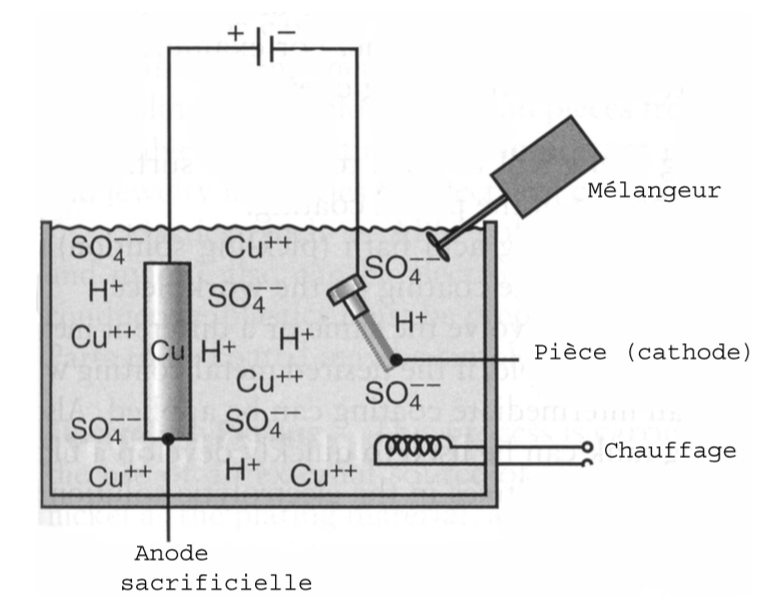
\includegraphics[scale=0.45]{electro.png}
\caption{Principe d'électrodéposition}
\label{fig:couches}
\end{figure}

Ions métalliques produits à l'anode (électrode positive) déposés sur une pièce placée à la cathode (électrode négative) de la cellule d'électrolyse.

Réaction à la cathode : $M^{n+}+ne^- \rightarrow M$

Domaines d'utilisations : corrosion, conductivité électrique, dureté et résistance à l'usure, esthétique, ... (nb: très long, 75$\mu m$ par heure)

\subsection{Traitements de conversion : objectifs et types}
\begin{itemize}[label=$\bullet$]
\item Formation d'un film fin d'oxyde, de chromate ou de phosphate via procédé chimique ou électrochimique.
\item Mise en contact par immersion ou projection.
\item Objectifs : anticorrosion, préparation de surfaces avant peinture, résistance à l'usure, bonne répartition du lubrifiant, isolation électrique, esthétique,...
\item Types : chimique, phosphatation ou chromatation (film de protection) ; anodation, oxyde stable en surface, pièce placée à l'anode (esthétique + anticorrosion)
\end{itemize}

%Mise en page
\pagebreak

\subsection{Dépôt chimique en phase vapeur}
Réaction chimique entre différents gaz donc le produit se dépose sur la pièce.

\paragraph{Avantages}
\begin{enumerate}
\item Dépôt de matériaux réfractaires bien en dessous de leur température de fusion.
\item Contrôle de la taille du grain.
\item Faisable sous pression atmosphérique.
\end{enumerate}

\paragraph{Inconvénients}
\begin{enumerate}
\item Produits chimiques toxiques et corrosifs
\item Produits chimiques coûteux
\item Beaucoup de pertes de produits chimiques.
\end{enumerate}

\subsection{Dépôt physique en phase vapeur}
\paragraph{Principe}
Dépôt d'un film mince sur un substrat par évaporation ou pulvérisation cathodique dans une chambre sous vide.
\paragraph{Étapes}
\begin{enumerate}
\item Synthèse de la vapeur par chauffage par résistance ou par bombardement ionique (faisceau d'électron)
\item Transport de la vapeur sous le substrat
\item Condensation de la vapeur sur le substrat (une température un peu élevée encourage la diffusion du dépôt dans le substrat)
\end{enumerate}

\subsection{Technologies pour le dépôt physique en phase vapeur}
Évaporation sous vide (surtout pour les métaux).

Pulvérisation cathodique : plasma entre substrat et matériau à déposer. Des ions d'argon vont bombarder le matériau à déposer, qui sera alors éjecté sur le substrat. Cela ne s'applique pas uniquement aux métaux. Désavantage : faible vitesse de dépôt.

\subsection{Traitements de diffusion}
\paragraph{Types}
Cémentation, nitruration, chromisation, boruration.

\paragraph{Objectifs}
Augmenter la teneur en alliage près de la surface pour une meilleure résistance à l'usure.

\section{Chapitre VIII : Mise en forme des polymères}
\subsection{Caractéristiques des polymères}
\begin{itemize}[label=$\checkmark$]
\item Résistance à la corrosion
\item Peu conducteur (chaleur, électricité)
\item Facile à mettre en œuvre
\item Température de fusion faible, donc peu coûteux en énergie
\item Forme visqueuse, on peut facilement les déformer
\item Mélange d'additifs facile (couleur, propriétés chimiques/mécaniques,...)
\item Matériaux composites à matrice polymère (très résistant, ajout de fibre et autres particules)
\end{itemize}
\begin{itemize}[label=$\times$]
\item Rigidité 100 fois inférieure à celle des métaux à température ambiante et résistance 10 fois inférieure
\item Comportement mécanique et aspect variable dans le temps
\item Dimensionnellement instable
\end{itemize}

\subsection{Comment se présentent les polymères microscopiquement}
C'est un enchevêtrement de chaînes moléculaires (macromolécules) sur base d'un monomère organique. Dans le monomère, les liaisons sont covalentes (fortes). Les chaînes sont liées entre elles par des liaisons faibles (H, ioniques, VdW). 

La polymérisation détermine les caractéristiques du matériau (viscosité, densité, tenue mécanique, ...), facteurs : degré de polymérisation(longueur moyenne chaîne), macromolécules (linéaires ou ramifiées), possibilité de faire un copolymère.

La polymérisation précède la mise en forme mais la microstructure peut évoluer pendant la fabrication :
\begin{itemize}[label=$\bullet$]
\item Degré de cristallinité des thermoplastiques. Détermine l'arrangement topologique des macromolécules (amorphe(désordonné) >< cristallin (régulier))
\item Degré de réticulation des thermodurcissants et des élastomères (nombre de jonction entre les molécules)
\end{itemize}

%Mise en page
\pagebreak

\subsection{Thermoplastiques}
Ce sont les polymères les plus courants.
\begin{itemize}[label=$\bullet$]
\item La température n'influence pas la mise en forme, seule compte la vitesse de refroidissement.
\item Solides (mais fragiles) à température ambiante et fluides (visqueux) vers 100$\degree$C.
\item Peuvent subir des cycles de fusion (solidification répétées sans altérations des propriétés).
\item Température augmente, la malléabilité augmente (liaisons secondaires entre chaînes rompues en premier).
\item Semi-cristallins (biphasés)
\item Refroidissement $\rightarrow$ degré de cristallité augmente si chaînes linéaires, refroidissement lent, préalablement aligné.
\item Phase amorphe : transition vitreuse à $T_g <T_{fus}$. Le module élastique chute, comportement viscoélastique, temps de relaxation augmente, la température diminue, pas d'effet sur la densité.
\item Phase cristalline ne subit pas de transition vitreuse. Au dessus de $T_m$ le comportement devient viscoélastique, densité augmente au dessus de $T_{fus}$ et le coefficient de dilatation augmente aussi.
\end{itemize}

\subsection{Thermodurcissants}
\begin{itemize}[label=$\bullet$]
\item Réactions chimiques générant des liaisons covalentes entre les chaînes $\rightarrow$ réticulation.
\item Polymères amorphes : réponse mécanique isotrope (bonne tenue mécanique si la température augmente).
\item Bonne isolation thermique/électrique.
\item Réticulation : $T>T_g$, puis refroidissement. Si on redépasse $T_g$, le thermodurcissant se dégrade.
\end{itemize}

\subsection{Elastomères}
\begin{itemize}[label=$\bullet$]
\item Thermodurcissants peu rigides $\rightarrow$ support de grandes déformations.
\item Microstructure particulière, $T_g < T_{amb}$

$\hookrightarrow$ Polymères très réticulés dont les chaînes sont repliées sur elles-mêmes. Contraintes : les chaînes se déplient et s'alignent (entropie chute) ensuite retour à un niveau d'entropie maximum.
\item Vulcanisation = réticulation du caoutchouc en présence de sulfure.
\end{itemize}

\subsection{Extrusion des thermoplastiques et élastomères}
Ce processus consiste à pousser un polymère fondu au travers d'une filière à la sortie de laquelle il se solidifie pour former un long profilé de section constante $\rightarrow$ processus continu pour grandes séries.

Ce polymère est mis sous pression dans une extrudeuse :  vis sans fin qui en tournant remplit plusieurs fonctions : le transport, le chauffage, le mélange et la compression. Le rayon de la vis augmente, et donc la hauteur radiale du conduit hélicoïdal diminue. Le pas de la vis reste constant.

\paragraph{Fonctionnement}
\begin{enumerate}
\item Arrivée des pastilles dans l'extrudeuse (gravité).
\item Portées à $T_{fusion}$ grâce à la chaleur de frottement et l'énergie de déformation du polymère.
\item A la sortie, le polymère forme : des produits plats (feuilles, films refroidis par trempe) ; des profilés (creux si utilisation d'un mandrin, air soufflé pour maintenir la section creuse).
\end{enumerate}

Calandrage : si le polymère s'extrude moins facilement, le film est aminci lors du passage à grande vitesse entre des rouleaux qui le compriment et l'étirent. Les feuilles extrudées sont mises en forme par thermoformage (feuille chaude mise en contact avec une matrice froide).

\subsection{Point de fonctionnement d'une extrudeuse}
=> Débit de l'écoulement et pression à l'entrée de la filière.

\begin{itemize}[label=$\bullet$]
\item Sens de rotation de la vis opposé à l'avancement du polymère. Filière cylindrique de rayon $R_f$ et de largeur $L_f$.
\item Mouvement rotatif du cylindre par rapport à la vis : dans le sens d'avancement

$\hookrightarrow$ On considère que c'est le frottement du polymère contre la paroi intérieure du cylindre qui fait progresser la charge.
\end{itemize}
\begin{align*}
\dot{Q} &= \dfrac{\pi R_f^4}{8\eta L_f}\Delta p
\end{align*}
$\eta=$viscosité dynamique

\subsection{Sensibilité à la vitesse de déformation}
Lors du passage en filière, le polymère devient viscoélastique. Une partie de l'énergie est conservé au sein du polymère et est relachée en sortie.
2 effets de ce retour élastique non-négligeable par rapport aux métaux: \begin{itemize}
\item Gonflement en sortie de filière. Solution:  sortie adaptée, refroidissement en sortie, effort de traction.
\item Capacité à subir de très grandes déformations sans subir de striction.
\end{itemize}

\subsection{Moulages relatifs aux polymères}
\begin{itemize}
\item Moulage par injection: mouvement de vis alternatif qui pousse le polymère liquide dans un moule(en sortie directe de l'extrudeuse).
\item Moulage par transfert: idem mais pas en sortie directe d'extrudeuse, attente dans une chambre et injection sous pression.
\item Moulage par compressios: application d'une poudre dans un moule, compression chauffe pour permettre la mise en forme(polymérisation et réticulation). Moins de contraintes résiduelles mais plus lent.
\item Moulage rotationnel: permet la fabrication de pièces creuses. Liquéfaction de poudre projetée puis solidification lors du refroidissement.
\end{itemize}

\subsection{Mot sur les composites à matrice polymère}
But: accorder des propriétés nouvelles par l'ajout d'un matériau composite (augmentation rapport résistance/poids, ténacité). En général les fibres ajoutées sont bien plus résistantes que le polymère en lui-même qui a plus un rôle de liant. Les fibres soutiennent les efforts uniquement selon leur axe. Si celles-ci sont établies aléatoirement, on aura un matériau isotrope(>< anisotrope, ex: cadre de vélo).



\section{Chapitre IX : Frittage et fabrication additive}

\subsection{La métallurgie des poudres}

La métallurgie des poudres consiste à la production de poudres de métaux/alliages et la fabrications de pièces à partir de celles-ci. La  fabrication est composée d'une phase de compression (obtention du "vert")suivie d'un traitement thermo-mécanique nommé \textit{frittage}.
\subsubsection{Avantages}
\begin{itemize}[label=$\bullet$]
\item Possibilité de réaliser des pièces en alliage à très haut point de fusion à des températures plus raisonnables (tungstène, tantale, molybdène,..)
\item Permet de réaliser des pièces en composés complexes qu'il est impossible de réaliser sans un mélange de poudres.
\item Permet de produire des matériaux \textbf{poreux}. On obtient la densité souhaitée en ajustant le frittage. Les pièces poreuses sont utiles lors de l'utilisation de lubrifiants.
\item On obtient directement la forme désirée dans le \textbf{moule de compaction}, moule dans lequel très peu de matière est perdue (rendement de 97\%).
\item Tolérance de fabrication après frittage plus strictes qu'en moulage.
\end{itemize}

%MEP


\subsubsection{Inconvénients}

\begin{itemize}[label=$\bullet$]
\item Coût des poudres et des moules de compaction très élevés. Approprié pour les grandes séries.
\item Sécurité plus importantes : risque de réactions poudres/air provoquant un incendie.
\item Contraintes géométriques (remplissage du moule et éjection de la pièce).
\item Densité de la pièce inhomogène si le remplissage du moule est mauvais
\item Production de petites pièces uniquement, 2kg maximum.
\end{itemize}

\subsubsection{Caractéristiques des poudres}

\begin{description}
\item[Taille]
De l'ordre du $\mu m$, elle est facilement définissable si la particule est sphérique. dans le cas contraire on utilise un tamis. Une poudre comportant des particules de tailles variables assure une bonne densité.
\item[Facteur de forme] Rapport entre la plus grande dimension et la plus petite dimension d'une particule. Plus difficile à déterminer avec des particules de formes complexes.

\item[Facteur d'écoulement] Mesure normée de la fluidité des poudres. Mesuré comme le temps nécessaire à l'écoulement de 50g de poudre au travers un entonnoir calibré de dimension normalisée.
\item[Composition chimique] La poudre peut être élémentaire (un seul élément du tableau périodique) ou pré-alliée
\end{description}

\subsubsection{Élaboration des pousses}

\begin{description}
\item[Atomisation]
Désintégration en petites gouttelettes d'un métal liquide sous l'action d'un \textbf{gaz inerte} ou d'\textbf{eau}. Méthode la plus répandue, elle permet de produire n'importe quel métal/alliage sous la forme de poudre de taille variable en fonction de la pression du jet. 

\begin{itemize}[label=$\square$]
\item Atomisation par jet d'eau : vitesse de refroidissement élevée ($10^3 \cdot \degree$C/s) et meilleure productivité. 

\item Atomisation par jet de gaz inerte : évite la formation d'une couche d'oxyde.

\item Atomisation centrifuge : Projection de métal fondu sur une un plateau refroidi tournant à haute vitesse. Vitesse de refroidissement excellente ($10^6 \cdot  \degree$C/s), permet de produire des poudres amorphes.
\end{itemize}
\item[Procédés chimiques]
On va distinguer différentes réactions chimiques :
	\begin{itemize}[label=$\bullet$]
		\item Réduction des poudres d'oxydes : (Fe, Cu, Ni, Co, Mo ou W) S'effectue en phase gazeuse (avec H,CO ou CH$_4$). L'agent réducteur va se recombiner avec l'oxygène de l'oxyde pour libérer le métal. Les poudres d'oxydes sont alors produites par broyage. Le broyage est plus aisé car les oxydes sont plus fragiles que les métaux purs (ductiles). On obtient généralement des poudres poreuses.
        \item Précipitation : (Cu, Ni ou Co) Action de l'HCL dans une solution du sulfate correspondant.
        \item Décomposition de composés carbonyles : (Fe ou Ni) Réaction du métal à haute pression et haute température pour former des composés volatils qui sont ensuite condensés sous forme liquie à température ambiante afin de former de fins cristaux. En chauffant à 250 $\degree$C on dissocie l'élément métallique du CO qui pourra être recyclé. Ce procédé permet d'obtenir des poudres très fines (quelques $\mu$m), quasi sphériques d'une très grande pureté.
\end{itemize}
    
\item[Dépot électrolytique] (Be, Cu, Fe, Ag, Ta, Ti) On effectue une électrolyse en plaçant le métal sous forme solide à l'anode et une solution aqueuse ou un sel fondu à la cathode. Cette technique produit des poudres \textbf{remarquablement pures}

\item[Broyage] Dans un premier temps, permet de réduire la taille des poudres fragiles (à l'aide d'un broyeur à cylindres, à marteaux ou d'un moulin à bille). Technique permettant de produire des \textbf{poudres céramiques}. 

Dans un second temps, à l'aide du moulin à bille, on peut procéder à \textbf{l'alliage mécanique des poudres} : on place  des poudres différentes et la succession d'écrasements, ruptures et micro soudages couplés à la diffusion produit des poudres alliées.
\end{description}

\subsubsection{Compaction}

Le produit obtenu après compaction des poudre est le \textbf{vert}. Le but de la compaction est de réduire la porosité initiale de l'amas de poudre et produire un ensemble manipulable pour le frittage. Le vert est assez fragile ($\approx$ craie) et risque de s'émietter/se rompre.

La \textit{densité} du vert est proportionnelle à la pression. Si la pression est suffisante, la déformation plastique des particules est possible, ce qui assure une bonne densité après frittage.

La \textit{cohésion} du vert est assurée par la déformation plastique ou l'ancrage mécanique entre les particules et la poudre. L'ancrage est favorisé par l'irrégularité de forme des particules. On peut rajouter un liant (qui sera supprimé au frittage) si la résistance du vert est trop fragile pour qu'il soit manipulé.

La pression requise à la compaction varie en fonction de l'alliage (de 70 à 800 Mpa), elle a lieu dans une \textbf{presse simple ou à multiples effets}. 
La tolérance y est très sévère (<25$\mu$m) afin d'évier les infiltrations de poudres. On utilise des presses \textbf{mécanique} pour les pressions <150 tonnes et des presses \textbf{hydraulique} sinon (5000 tonnes max). Les presses à effets multiples permettent la compaction de pièces complexes et donnent une meilleure densité au vert. On peut incorporer un lubrifiant qui peut également faire office de liant afin de réduire les frottements.

La \textbf{compression isostatique à froid} donne une densité plus uniforme. On applique une pression isostatique sur un moule flexible (généralement de l'eau sur un moule en plastique). De l'ordre de 400 MPa on n'obtient pas des tolérances très serrées et des opérations de finition sont parfois nécessaires.

\subsubsection{Frittage}

Cette opération consiste à porter le vert à haute température (0.7 à 0.8 fois la température de fusion) sous atmosphère contrôlée afin d'établir des liaisons entre particules et donner au produit fritté les propriétés classiques de l'état métallique (résistance, ductilité, conductivité,..). On doit contrôler l'atmosphère pour éviter l'oxydation du vert et pouvoir contrôler la carburation des verts à base de fer. 

Le frittage va faire diminuer les surfaces libres et augmenter la densité. Certains constituant des poudres ayant une température de fusion inférieur à celle du processus peuvent fondre et s'écouler dans les porosités.

%MEP
\pagebreak

Le frittage classique se fait dans des fours continus comme suit : 
\begin{enumerate}
\item Zone de préchauffage : sèche le vert et élimine les liants.
\item Zone à haute température : pour le frittage.
\item Zone de refroidissement. 
\end{enumerate}

\subsubsection{Compaction \& Frittage}
\begin{description}
\item[Pressage à chaud :] Un cycle thermique est appliqué à la pièce en cours de compaction. La densité obtenue est plus grande grâce à l'utilisation de la déformation plastique à chaud.
\item[Compaction isostatique à chaud :] De la même manière que le procédé à froid, on va utiliser cette fois un moule pouvant résister à de très grandes températures et le fluide ne sera plus de l'eau mais un gaz inerte. Les pièces issus de ce procédé ont densité proche de 100\% et une excellente homogénéité néanmoins ce procédé est lent et très coûteux !
\item[Frittage flash :] Combine le passage d'un courant continu ou pulsé à travers la matrice d'une presse à chaud et à travers la poudre si elle est conductrice. La chaleur est donc générée \textbf{intérieurement}, ce qui permet des vitesses de chauffe plus élevées : les temps de cycles sont plus courts ce qui évite la croissance des grains.
\item[Procédés classiques :] Le \textbf{laminage} des poudres permet de compacter en continu les poudres. Le frittage peut être réalisé par après. Les tôles obtenus ont une bonne densité. La compaction et le frittage peuvent être réalisé en une seule étape par \textbf{extrusion ou forgeage à chaud}
\end{description}
\subsection{Fabrication de pièce céramique}
On retrouve des céramiques \textit{techniques} dans le domaine médical, les outils de coupe, les combustibles nucléaires et les substrats pour circuits électroniques.

Les poudres céramiques sont broyées en une poudre très finies et sont assemblée par un additif :
\begin{itemize}[label=$\bullet$]
\item plastifiant : Améliore la capacité de la pate assemblée à rentrer dans le moule.
\item Liant : tenir les particules de céramiques ensemble
\item Agent mouillant : obtenir un meilleur mélange.
\item Défloculant : éviter un encastrement ou des jonctions prématurées entre particules.
\item Lubrifiant : réduire les frottements entre particules et aider au démoulage.
\end{itemize}

La pâte additif/poudre est ensuite fritée à une température de 0.9 à 0.9 fois la température de fusion de la céramique. Selon les mêmes procédés que pour les métaux.

%MEP
\pagebreak

\subsection{Fabrication additive}

Utilisée pour le \textbf{prototypage rapide} la fabrication additive consiste en la construction d'une pièce couche par couche avec des tranches d'épaisseurs variables ($[10^{-5};10^{-4}] m$).

Les technologies de fabrication additives sont\footnote{Copié-collé du syllabus, tout y es dis.} :
\begin{description}
\item[Modélisation par dépôt de fils en fusion FDM :] Consiste à extruder un filament d’un matériau thermoplastique à travers un fin orifice chauffé à l’aide d’un robot qui se déplace selon l’endroit où il convient de déposer de la matière. La table descend lorsqu’une tranche est terminée. La pièce est initialement construite sur une table en mousse de polymère qui sera ensuite séparée de la pièce. Les supports de pièces qui ne sont pas auto-portants sont également construits par extrusion mais avec un maillage beaucoup plus grossier afin que la pièce soit moins dense à ces endroits-là et ainsi se détachent facilement lorsque la pièce est terminée. Les tolérances des pièces peuvent atteindre 0.02 mm, (cette technologie peut s’appliquer aussi aux métaux qui sont alors fondus par un laser).
\item[Stéréolithographie] basée sur le principe de la polymérisation d’un photopolymère par action de la lumière. La résine utilisée est généralement un mélange de monomères acrylates ou époxys et d’un photoinitiateur. Le rôle du photoinitiateur est d’initier la polymérisation du matériau sous l’effet de la lumière. Un laser fixe générant un rayon ultra-violet est focalisé en surface du bassin contenant le photopolymère à l’aide de déflecteurs qui permettent de déplacer le faisceau à l’endroit souhaité. Lorsqu’une tranche est finalisée, la plateforme descend afin d’exécuter la tranche suivante. La dernière étape est la cuisson de la pièce. La matière non utilisée après la fabrication de la pièce peut servir à la pièce suivante. Les tolérances des pièces peuvent atteindre 0.01 mm.

\item[Impression à jets multiples :] On utilise aussi un photopolymère qui est injecté à l’endroit souhaité construisant ainsi la pièce couche par couche. Ici la cuisson du polymère se fait en cours de production et il n’y a pas d’étape supplémentaire comme en stéréolithographie. L’imprimante a deux têtes (ou plus) d’impression : une pour la pièce et l’autre pour le matériau de support. Le support est réalisé dans un gel qui peut facilement être retiré par simple nettoyage dans une solution aqueuse. Il est possible de rajouter des têtes avec des couleurs différentes. Un exemple d’application de ce genre d’imprimante 3D est dans la réalisation de maquette d’architecte.
\item[Fusion sélective laser SLM]

On utilise un laser pour fondre (ou fritter) des poudres plastiques ou métalliques et ainsi construire des pièces 3D. Cette technologie est particulièrement intéressante pour réaliser des pièces métalliques impossible à réaliser avec les technologies limitées aux polymères. Un rouleau racleur dépose alors une couche de poudre métallique sur une plateforme qui descend au fur et à mesure que le laser fond ou fritte la pièce dans sa forme souhaitée. A la fin du processus la pièce est noyée dans de la poudre et doit donc être nettoyée mais l’excès de poudre peut être recyclé. La fusion par faisceau d’électrons assure la fusion. Un faisceau d’électron est beaucoup plus efficace d’un point de vue énergétique qu’un faisceau laser (95\% de l’énergie est utilisée pour fondre alors que 10-20\% seulement en technologie SLM). Il est donc plus facile d’arriver à la fusion plutôt qu’au frittage des poudres.
\end{description}

\newpage

\appendix

\section{Liens Youtubes}

\subsection{Mise en forme}

\subsubsection*{Moulage des métaux}
\begin{itemize}
 \item \url{http://www.youtube.com/watch?feature=player_detailpage&v=IrcNSgLZuFs}
 \item \url{http://www.youtube.com/watch?feature=player_detailpage&v=dOw624I9FDQ}
 \item \url{http://www.youtube.com/watch?v=K8SYhISGxN4&list=PLi1MY42ijrYEahnUoaL7xxS96Cpkt1MX}
\end{itemize}

\subsubsection*{Mise en forme des polymères et composites}
\begin{itemize}
 \item \url{http://www.youtube.com/watch?feature=player_detailpage&v=QR4Aa671aHE}
 \item \url{http://www.youtube.com/watch?feature=player_detailpage&v=wANlQCozCSQ}
 \item \url{http://www.youtube.com/watch?feature=player_detailpage&v=MD7TiUoaB8}
 \item \url{http://www.youtube.com/watch?feature=player_detailpage&v=eUthHS3MTdA}
 \item \url{http://web.empreinte.com/webtv/michelin/tslp-fabrication-pneu-fr-20131029.mp4}
 \item \url{http://www.youtube.com/watch?feature=player_detailpage&v=NPLWxxyIJcE}
\end{itemize}

\subsubsection*{Extrusion des métaux}
\begin{itemize}
 \item \url{http://www.youtube.com/watch?feature=player_detailpage&v=vHkwq_2yY9E}
 \item \url{http://www.youtube.com/watch?feature=player_detailpage&v=iiGlq7408ME}
 \item \url{http://www.youtube.com/watch?feature=player_detailpage&v=LnDUYZHDQAg}
\end{itemize}

\subsubsection*{Forgeage des métaux}
\begin{itemize}
 \item \url{http://www.youtube.com/watch?feature=player_detailpage&v=OaAcfpWnfh4}
 \item \url{http://www.youtube.com/watch?feature=player_detailpage&v=XTU0Z-FkhtU}
 \item \url{http://www.youtube.com/watch?feature=player_detailpage&v=6Gg0_putA5A}
\end{itemize}

\subsubsection*{Tréfilage}
\begin{itemize}
 \item \url{http://www.youtube.com/watch?feature=player_detailpage&v=YlLWBM2e5qg}
 \item \url{http://www.youtube.com/watch?feature=player_detailpage&v=o6m1Uii5v2I}
\end{itemize}

\subsubsection*{Étirage}
\begin{itemize}
 \item \url{http://www.youtube.com/watch?v=QKAg1yMZIpY}
 \item \url{http://www.youtube.com/watch?v=zlueIHudt4k}
\end{itemize}

\subsubsection*{Laminage}
\begin{itemize}
 \item \url{http://www.youtube.com/watch?feature=player_detailpage&v=7ITgMXtuMv0}
 \item \url{http://www.youtube.com/watch?feature=player_detailpage&v=AuuP8L-WppI}
 \item \url{http://www.youtube.com/watch?v=f4OTj9yNOak}
\end{itemize}

\subsubsection*{Pliage}
\begin{itemize}
 \item \url{http://www.youtube.com/watch?v=k6iODHla6qY}
 \item \url{http://www.youtube.com/watch?v=7Ojxha-Y-dg}
 \item \url{http://www.youtube.com/watch?feature=player_detailpage&v=qTUMbVNf1Xc}
\end{itemize}

\subsubsection*{Emboutissage}
\begin{itemize}
 \item \url{http://www.youtube.com/watch?feature=player_detailpage&v=V4TVDSWuR5E}
 \item \url{http://www.youtube.com/watch?v=hcsDxCagWrY}
 \item \url{http://www.youtube.com/watch?feature=player_detailpage&v=qTUMbVNf1Xc}
\end{itemize}

\subsection{Usinage}

\subsubsection*{Le métier d’usineur}
\begin{itemize}
 \item Général : \url{http://www.youtube.com/watch?v=ARJA1KRg5XI}
 \item Rectifieur : \url{http://www.youtube.com/watch?v=lWAF3NaR6pQ}
\end{itemize}

\subsubsection*{Tournage}
\begin{itemize}
 \item Découvrir un tour parallèle : \url{http://www.youtube.com/watch?v=WrsDUA6PKoM}
 \item Tronçonnage : \url{http://www.youtube.com/watch?v=vd1H843FtR0}
 \item Centrage : \url{http://www.youtube.com/watch?v=UYKL0Jk3Ycc}
 \item Perçage : \url{http://www.youtube.com/watch?v=RKAvnu0uLWY}
 \item Dressage sur série de pièces : \url{http://www.youtube.com/watch?v=z8oIhl1fkaY}
 \item Tour vertical : \url{http://www.youtube.com/watch?v=D21OfCcxdz4}
 \item Montage : \url{http://www.youtube.com/watch?v=Q7QUiCJJmew&list=PL7WrlP7eO7nZ--oAzc_1KURv_cftmZ6Sy}
\end{itemize}

\subsubsection*{Fraisage}
\begin{itemize}
 \item Découvrir une fraiseuse conventionnelle : \url{http://www.youtube.com/watch?v=JD1Kqw9vNTo}
 \item Surfaçage/dressage : \url{http://www.youtube.com/watch?v=MpHbpgsfuY0}
 \item Régler les butées de fin de course : \url{http://www.youtube.com/watch?v=jhPMwkbc_YE}
 \item Rainurage débouchant en ébauche : \url{http://www.youtube.com/watch?v=-p_uZA2X6GA}
\end{itemize}

\subsubsection*{Perçage}
\begin{itemize}
 \item Découvrir une perceuse sensitive : \url{http://www.youtube.com/watch?v=q_5pJZZ-b1w}
 \item Taraudage avec un outil à tarauder : \url{http://www.youtube.com/watch?v=tnfQX_gBh7c}
\end{itemize}

\subsubsection*{Rectifieuse}
\begin{itemize}
 \item Plane : \url{http://www.youtube.com/watch?v=cSw4Lu_paXw}
 \item \url{http://www.youtube.com/watch?v=qGv4QQNYj6U}
 \item Centerless : \url{http://www.youtube.com/watch?v=S7nDiCqocVc}
\end{itemize}

\subsubsection*{Raboteuse}
\begin{itemize}
 \item \url{http://www.youtube.com/watch?v=sVRwK5e2178}
 \item \url{http://www.youtube.com/watch?v=vWodXc-2U3w}
\end{itemize}

\subsection{Métallurgie des poudres et fabrication additive}

\begin{itemize}
 \item Atomisation au gaz : \url{https://www.youtube.com/watch?v=ldP1sQnjWcc}
 \item Compaction + Frittage conventionnels : \url{https://www.youtube.com/watch?v=O7U4HWjYcqo}
 \item Compaction isostatique à chaud : \url{https://www.youtube.com/watch?v=dysqMX3amhU}
 \item Fabrication additive : dépôt de fil en fusion : \url{https://www.youtube.com/watch?v=WHO6G67GJbM}
 \item Fabrication additive : electron beam melting (EBM) : \url{https://www.youtube.com/watch?v=GjbkxVku39Y}
 \item Fabrication additive: perspective industrielles : \url{https://www.youtube.com/watch?v=l0SXlkrmzyw}
\end{itemize}

\subsection{Assemblage}

\begin{itemize}
 \item Soudage laser : \url{https://www.youtube.com/watch?v=Gsj44ObhL24}
 \item Soudage par explosion : \url{https://www.youtube.com/watch?v=2u51tJdRDK0}
 \item Soudage par friction inertielle : \url{https://www.youtube.com/watch?v=-aEuAK8bsQg}
\end{itemize}

\subsection{Physique de la déformation plastique}

\begin{itemize}
 \item Modélisation par dynamique moléculaire de l’interaction entre une dislocation et une cavité : \url{https://www.youtube.com/watch?v=ESywdADUBDU}
 \item Interaction entre une dislocation et un atome en solution solide : \url{https://www.youtube.com/watch?v=RUuLusenhfA}
 \item Module de Young/Limite d’élasticité/Effet des joints de grains/Fragilité des céramiques : \url{https://www.youtube.com/watch?v=J3DljAG0QcI}
\end{itemize}

\subsection{Traitements de surface}

\subsubsection*{Grenaillage}
\begin{itemize}
 \item \url{https://www.youtube.com/watch?v=FxFiyCVk21s}
\end{itemize}

\end{document}
